\documentclass[11pt,letterpaper]{article}
\usepackage[T1]{fontenc}
\usepackage[utf8]{inputenc}
\usepackage{lmodern}
\usepackage[margin=1in]{geometry}
\usepackage{graphicx}
\usepackage{float}
\usepackage{longtable}
\usepackage{array}
\usepackage{xcolor}
\usepackage{listings}
\usepackage[hidelinks]{hyperref}

\setlength{\parindent}{0pt}
\setlength{\parskip}{6pt}
\setlength{\emergencystretch}{3em}
\renewcommand{\arraystretch}{1.15}

\lstset{
  basicstyle=\ttfamily\footnotesize,
  breaklines=true,
  columns=fullflexible,
  frame=single,
  framerule=0.3pt,
  rulecolor=\color{black!40},
  xleftmargin=0pt,
  aboveskip=6pt,
  belowskip=6pt
}

% inline code: typewriter, with places where a long name may break
\newcommand{\code}[1]{\texttt{#1}}
% a screenshot that has not been captured yet (still counts as a figure number)
\newcommand{\pendingfigure}[2]{%
  \refstepcounter{figure}%
  \begin{center}
  \fbox{\parbox{0.9\linewidth}{\centering\textbf{\textcolor{red!70!black}{SCREENSHOT PENDING}}\\[2pt]
  \texttt{#1}\\[2pt] Figure \thefigure: #2}}
  \end{center}}

\begin{document}
\begin{center}
{\LARGE\bfseries DATA-260 Lab 1 -- Report}\\[6pt]
{\large \textbf{Pair 06} $\cdot$ Uday Patel (Part A) and Sreeramachandra Sai Achutuni (Parts B and C)}
\end{center}


{\small
\begin{longtable}{>{\raggedright\arraybackslash}p{\dimexpr 0.191\linewidth-2\tabcolsep\relax}>{\raggedright\arraybackslash}p{\dimexpr 0.809\linewidth-2\tabcolsep\relax}}
\hline
\textbf{Item} & \textbf{Value} \\ \hline
\endhead
Repository & \url{https://github.com/UdayPate/data260-pair06} (private) \\ \hline
Tagged commit & \code{<!-\allowbreak{}-\allowbreak{} FILL AT THE END:\allowbreak{} final commit hash,\allowbreak{} tag lab1 -\allowbreak{}-\allowbreak{}>} \\ \hline
Hardware & Lenovo Legion Slim 5 (16-inch, Ryzen 5 7640HS, 16 GB RAM, RTX 4060 8 GB), Windows, MySQL 8 local \\ \hline
Local model & \code{qwen3:\allowbreak{}8b} via Ollama (Parts B and C) \\ \hline
\end{longtable}
}

\section*{Section 1 -- Goals}

Lab 1 asks for a Handshake-style career platform with two personas, \textbf{Student} and \textbf{Company}, and a hand-built AI assistant that works on the platform's own data. The platform uses React (front end), FastAPI (back end) and MySQL (database). The assistant uses a local Ollama model and an agent loop written by hand, with no agent framework. The lab is worth 40 points.

{\small
\begin{longtable}{>{\raggedright\arraybackslash}p{\dimexpr 0.081\linewidth-2\tabcolsep\relax}>{\raggedright\arraybackslash}p{\dimexpr 0.743\linewidth-2\tabcolsep\relax}>{\raggedleft\arraybackslash}p{\dimexpr 0.081\linewidth-2\tabcolsep\relax}>{\raggedright\arraybackslash}p{\dimexpr 0.095\linewidth-2\tabcolsep\relax}}
\hline
\textbf{Part} & \textbf{What it asks for} & \textbf{Points} & \textbf{Owner} \\ \hline
\endhead
A & The platform: both personas, REST API, validation, authorization, Swagger or Postman documentation, seed generator & 22 & Uday \\ \hline
B & Agent loop, one model client class, five tools, five transcripts & 12 & Partner \\ \hline
C & Confirmation gate, prompt-injection defence, tool-call reliability table & 6 & Partner \\ \hline
\end{longtable}
}

This report covers all three parts. Sections 1 to 6 are Part A. Sections 7 to 10 are Parts B and C.

The goals for Part A, taken from the handout:

\begin{itemize}
\item \textbf{Student:} sign up (bcrypt) and sign in/out with a token; profile with every updatable field and a picture; search jobs by company or title and filter by category and city; job and company details; apply with a PDF resume and filter own applications by Pending, Reviewed or Declined; events in date order, search, register when eligible; browse students by name or college and filter by major; AI chat on the home page.
\item \textbf{Company:} sign up and sign in/out; post jobs; see own postings and who applied; open a student profile, preview the PDF resume and set the status; company profile with picture; Students tab (name, college, skills); Events tab (post events, see registered students).
\item \textbf{Back end and front end:} validate every input, encrypt passwords, handle exceptions, restrict users to authorized actions; React with Bootstrap, Axios, loading and error states, separate components, pages and services; Swagger UI or a Postman collection.
\item \textbf{Data:} at least 300 jobs, 1,500 applications, 200 students, 50 companies and 100 events across CITY\_SET, generated with \code{random\_\allowbreak{}state =\allowbreak{} SEED} by a committed script.
\end{itemize}

How we know each goal is met: the requirement-to-code-to-test table is in \code{docs/\allowbreak{}PART\_\allowbreak{}A\_\allowbreak{}CHECKLIST.\allowbreak{}md}, the API evidence is in section 6, and the test counts are in section 6 and \code{METRICS.\allowbreak{}md}.

\section*{Section 2 -- System design}

\subsection*{2.1 -- Architecture}

\begin{lstlisting}
 Browser  (React 18 + Vite + react-bootstrap, http://localhost:9061)
    |  pages -> services/*.js -> services/api.js (Axios, adds the token, one place for errors)
    v  HTTP + JSON, header  Authorization: Bearer <JWT>
 FastAPI  (http://localhost:9060, Swagger UI at /docs)
    routers/    HTTP only: path, status code, which role may call it
    schemas/    Pydantic v2: validates every request body and shapes every response
    services/   business rules and queries (jobs, events, students, preferences, applications)
    models.py   SQLAlchemy 2.0 tables
    |            ^
    |            +-- services/ is also what the AI assistant tools call (Parts B and C),
    v                so the assistant gets the same permission rules as the website
 MySQL 8  (database p06_handshake)       uploads/  (resumes: private; profile_pics: public)
\end{lstlisting}

JWT = JSON Web Token. CORS (Cross-Origin Resource Sharing) allows only the React origin (port 9061).

\subsection*{2.2 -- Layers and why they are split}

{\small
\begin{longtable}{>{\raggedright\arraybackslash}p{\dimexpr 0.082\linewidth-2\tabcolsep\relax}>{\raggedright\arraybackslash}p{\dimexpr 0.271\linewidth-2\tabcolsep\relax}>{\raggedright\arraybackslash}p{\dimexpr 0.647\linewidth-2\tabcolsep\relax}}
\hline
\textbf{Layer} & \textbf{Folder} & \textbf{Rule it follows} \\ \hline
\endhead
Router & \code{backend/\allowbreak{}app/\allowbreak{}routers/\allowbreak{}} & Thin. Reads the request, calls one service function, returns the result. \\ \hline
Schema & \code{backend/\allowbreak{}app/\allowbreak{}schemas/\allowbreak{}} & Every request body is a Pydantic model that checks types, lengths and ranges. The job, event, preference, profile-update, status-update and chat bodies also use \code{extra=\allowbreak{}"forbid"}, so an unknown field such as \code{company\_\allowbreak{}id} gets 422. The signup and login bodies do not forbid extra fields; unknown fields there are ignored and never reach the database. \\ \hline
Service & \code{backend/\allowbreak{}app/\allowbreak{}services/\allowbreak{}} & All business rules and SQL. The website and the assistant call the same functions. \\ \hline
Model & \code{backend/\allowbreak{}app/\allowbreak{}models.\allowbreak{}py} & Table definitions, enums, UNIQUE constraints. \\ \hline
Core & \code{backend/\allowbreak{}app/\allowbreak{}core/\allowbreak{}} & Password hashing, JWT, role checks (\code{deps.\allowbreak{}py}), safe uploads. \\ \hline
\end{longtable}
}

Front end: pages never call Axios directly. Pages call \code{services/\allowbreak{}*.\allowbreak{}js}, which call \code{services/\allowbreak{}api.\allowbreak{}js}. The \code{useAsync} hook gives every request a loading state, an error state and a reload. Array filters are sent as repeated keys (\code{paramsSerializer:\allowbreak{} \{ indexes:\allowbreak{} null \}}), which is what FastAPI expects.

\subsection*{2.3 -- Data model}

Twelve tables (all in \code{backend/\allowbreak{}app/\allowbreak{}models.\allowbreak{}py}):

{\small
\begin{longtable}{>{\raggedright\arraybackslash}p{\dimexpr 0.257\linewidth-2\tabcolsep\relax}>{\raggedright\arraybackslash}p{\dimexpr 0.372\linewidth-2\tabcolsep\relax}>{\raggedright\arraybackslash}p{\dimexpr 0.372\linewidth-2\tabcolsep\relax}}
\hline
\textbf{Table} & \textbf{Purpose} & \textbf{Notable constraints} \\ \hline
\endhead
\code{students} & Student account and profile & \code{email} unique, \code{password\_\allowbreak{}hash} (bcrypt) \\ \hline
\code{student\_\allowbreak{}skills}, \code{student\_\allowbreak{}experience} & Skills and work history & skill unique per student; cascade delete \\ \hline
\code{student\_\allowbreak{}preferences} & Saved job and event preferences (read by the assistant) & one row per student \\ \hline
\code{companies} & Company account and profile & \code{email} unique \\ \hline
\code{jobs}, \code{job\_\allowbreak{}skills} & Postings and required skills & enums for category and pay period; skill unique per job \\ \hline
\code{applications} & A student applying to a job, with resume path and status & UNIQUE (\code{student\_\allowbreak{}id}, \code{job\_\allowbreak{}id}) \\ \hline
\code{events}, \code{event\_\allowbreak{}eligible\_\allowbreak{}majors} & Events and the majors allowed (one row \code{All} = open to everyone) & UNIQUE (\code{event\_\allowbreak{}id}, \code{major}) \\ \hline
\code{event\_\allowbreak{}registrations} & A student registered for an event & UNIQUE (\code{student\_\allowbreak{}id}, \code{event\_\allowbreak{}id}) \\ \hline
\code{saved\_\allowbreak{}items} & Jobs or events saved by the assistant's \code{save\_\allowbreak{}job\_\allowbreak{}or\_\allowbreak{}event} tool & UNIQUE (\code{student\_\allowbreak{}id}, \code{item\_\allowbreak{}type}, \code{item\_\allowbreak{}id}) \\ \hline
\end{longtable}
}

In this report a \textbf{job posting} is a row in \code{jobs} (the API paths say \code{/\allowbreak{}jobs}). Relationships: a company has many job postings and events; a job has many applications; a student has many applications and registrations. Foreign keys use \code{ON DELETE CASCADE}. Application status is the enum Pending, Reviewed, Declined; job category is the enum full\_time, part\_time, on\_campus, internship.

\subsection*{2.4 -- Authentication}

\begin{itemize}
\item Passwords are hashed with bcrypt (the library's default cost, 12 rounds; \code{core/\allowbreak{}security.\allowbreak{}py}). At least 8 characters, one letter and one digit, at most 72 bytes (the bcrypt limit). The hash is never returned by any endpoint.
\item \code{POST /\allowbreak{}auth/\allowbreak{}login} returns a JWT (HS256, 8 hours) that holds the user id, the role and the expiry. The client sends it as \code{Authorization:\allowbreak{} Bearer <token>}. A wrong email and a wrong password give the same reply (\code{test\_\allowbreak{}login\_\allowbreak{}wrong\_\allowbreak{}password\_\allowbreak{}and\_\allowbreak{}unknown\_\allowbreak{}email\_\allowbreak{}look\_\allowbreak{}identical}).
\item \code{core/\allowbreak{}deps.\allowbreak{}py} turns the token into the current user. A missing, forged or expired token gives \textbf{401}. \code{require\_\allowbreak{}student} and \code{require\_\allowbreak{}company} give \textbf{403} to the wrong role.
\item The JWT secret and the database password come from \code{backend/\allowbreak{}.\allowbreak{}env}, which is git-ignored.
\end{itemize}

\subsection*{2.5 -- Authorization and role rules}

{\small
\begin{longtable}{>{\raggedright\arraybackslash}p{\dimexpr 0.333\linewidth-2\tabcolsep\relax}>{\raggedright\arraybackslash}p{\dimexpr 0.333\linewidth-2\tabcolsep\relax}>{\raggedright\arraybackslash}p{\dimexpr 0.333\linewidth-2\tabcolsep\relax}}
\hline
\textbf{Rule} & \textbf{Behaviour} & \textbf{Test that checks it} \\ \hline
\endhead
Missing, garbage, expired, wrongly signed token, or deleted account & \textbf{401} & \code{test\_\allowbreak{}auth.\allowbreak{}py:\allowbreak{}:\allowbreak{}test\_\allowbreak{}missing\_\allowbreak{}or\_\allowbreak{}garbage\_\allowbreak{}token\_\allowbreak{}is\_\allowbreak{}401}, \code{test\_\allowbreak{}expired\_\allowbreak{}token\_\allowbreak{}is\_\allowbreak{}401}, \code{test\_\allowbreak{}token\_\allowbreak{}signed\_\allowbreak{}with\_\allowbreak{}wrong\_\allowbreak{}secret\_\allowbreak{}is\_\allowbreak{}401}, \code{test\_\allowbreak{}token\_\allowbreak{}for\_\allowbreak{}deleted\_\allowbreak{}account\_\allowbreak{}is\_\allowbreak{}401} \\ \hline
A user's own data & Always taken from the token (\code{/\allowbreak{}students/\allowbreak{}me}), never from an id in the URL & By design (the routes have no id); no single test is named for it \\ \hline
Another person's resume & \textbf{404}, not 403, for another student, for a company that does not own the job, and for an id that does not exist (same reply body); 401 when not logged in & \code{test\_\allowbreak{}applications.\allowbreak{}py:\allowbreak{}:\allowbreak{}test\_\allowbreak{}everyone\_\allowbreak{}else\_\allowbreak{}gets\_\allowbreak{}404\_\allowbreak{}for\_\allowbreak{}a\_\allowbreak{}resume} \\ \hline
Another company's application & \code{GET /\allowbreak{}applications/\allowbreak{}\{id\}} gives \textbf{404}; a student calling that company-only endpoint gets \textbf{403} & \code{test\_\allowbreak{}applications.\allowbreak{}py:\allowbreak{}:\allowbreak{}test\_\allowbreak{}applicant\_\allowbreak{}detail\_\allowbreak{}privacy} \\ \hline
Applicants list of a job posting the company does not own & \textbf{403} (the posting itself is public, so its existence is not secret); a student gets 403; a missing posting is 404 & \code{test\_\allowbreak{}applications.\allowbreak{}py:\allowbreak{}:\allowbreak{}test\_\allowbreak{}applicants\_\allowbreak{}list\_\allowbreak{}is\_\allowbreak{}private\_\allowbreak{}to\_\allowbreak{}the\_\allowbreak{}job\_\allowbreak{}owner} \\ \hline
Company editing a job posting or event it does not own & \textbf{403} & \code{test\_\allowbreak{}jobs.\allowbreak{}py:\allowbreak{}:\allowbreak{}test\_\allowbreak{}cannot\_\allowbreak{}edit\_\allowbreak{}someone\_\allowbreak{}elses\_\allowbreak{}job\_\allowbreak{}or\_\allowbreak{}a\_\allowbreak{}missing\_\allowbreak{}job}, \code{test\_\allowbreak{}events.\allowbreak{}py:\allowbreak{}:\allowbreak{}test\_\allowbreak{}cannot\_\allowbreak{}edit\_\allowbreak{}someone\_\allowbreak{}elses\_\allowbreak{}event\_\allowbreak{}or\_\allowbreak{}a\_\allowbreak{}missing\_\allowbreak{}one} \\ \hline
Event registration when the student's major is not eligible (or the student has no major and the event is not open to all) & \textbf{403} with the reason in the message & \code{test\_\allowbreak{}events.\allowbreak{}py:\allowbreak{}:\allowbreak{}test\_\allowbreak{}ineligible\_\allowbreak{}student\_\allowbreak{}is\_\allowbreak{}refused\_\allowbreak{}with\_\allowbreak{}a\_\allowbreak{}clear\_\allowbreak{}reason}, \code{test\_\allowbreak{}student\_\allowbreak{}without\_\allowbreak{}a\_\allowbreak{}major\_\allowbreak{}can\_\allowbreak{}only\_\allowbreak{}join\_\allowbreak{}open\_\allowbreak{}events} \\ \hline
Registering for a past event & \textbf{409} & \code{test\_\allowbreak{}events.\allowbreak{}py:\allowbreak{}:\allowbreak{}test\_\allowbreak{}cannot\_\allowbreak{}register\_\allowbreak{}for\_\allowbreak{}past\_\allowbreak{}or\_\allowbreak{}missing\_\allowbreak{}events\_\allowbreak{}or\_\allowbreak{}as\_\allowbreak{}other\_\allowbreak{}roles} \\ \hline
Duplicate application, duplicate registration, signup with an existing email & \textbf{409} (the UNIQUE constraint is the final guard against two clicks at once) & \code{test\_\allowbreak{}applications.\allowbreak{}py:\allowbreak{}:\allowbreak{}test\_\allowbreak{}cannot\_\allowbreak{}apply\_\allowbreak{}twice\_\allowbreak{}but\_\allowbreak{}can\_\allowbreak{}apply\_\allowbreak{}to\_\allowbreak{}other\_\allowbreak{}jobs}, \code{test\_\allowbreak{}events.\allowbreak{}py:\allowbreak{}:\allowbreak{}test\_\allowbreak{}cannot\_\allowbreak{}register\_\allowbreak{}twice\_\allowbreak{}but\_\allowbreak{}others\_\allowbreak{}can}, \code{test\_\allowbreak{}auth.\allowbreak{}py:\allowbreak{}:\allowbreak{}test\_\allowbreak{}duplicate\_\allowbreak{}email\_\allowbreak{}is\_\allowbreak{}rejected\_\allowbreak{}case\_\allowbreak{}insensitively} \\ \hline
Resumes & Private. Served only by \code{GET /\allowbreak{}applications/\allowbreak{}\{id\}/\allowbreak{}resume} to the applicant and the owning company, with \code{Cache-\allowbreak{}Control:\allowbreak{} private,\allowbreak{} no-\allowbreak{}store}; the resumes folder is not mounted as static files & \code{test\_\allowbreak{}resume\_\allowbreak{}files\_\allowbreak{}are\_\allowbreak{}not\_\allowbreak{}served\_\allowbreak{}as\_\allowbreak{}static\_\allowbreak{}files}, \code{test\_\allowbreak{}profiles.\allowbreak{}py:\allowbreak{}:\allowbreak{}test\_\allowbreak{}resumes\_\allowbreak{}folder\_\allowbreak{}is\_\allowbreak{}not\_\allowbreak{}publicly\_\allowbreak{}served} \\ \hline
Profile pictures & Public under \code{/\allowbreak{}media/\allowbreak{}profile\_\allowbreak{}pics/\allowbreak{}} & \code{test\_\allowbreak{}profiles.\allowbreak{}py:\allowbreak{}:\allowbreak{}test\_\allowbreak{}upload\_\allowbreak{}picture\_\allowbreak{}and\_\allowbreak{}serve\_\allowbreak{}it} \\ \hline
What a company sees of a student in the \textbf{list} (\code{GET /\allowbreak{}students}) & Name, college, major, degree, graduation year, skills, city, state, \textbf{email and GPA}; no phone, no date of birth & \code{test\_\allowbreak{}directory.\allowbreak{}py:\allowbreak{}:\allowbreak{}test\_\allowbreak{}company\_\allowbreak{}list\_\allowbreak{}shows\_\allowbreak{}contact\_\allowbreak{}and\_\allowbreak{}academic\_\allowbreak{}fields\_\allowbreak{}but\_\allowbreak{}never\_\allowbreak{}dob\_\allowbreak{}phone\_\allowbreak{}or\_\allowbreak{}password} \\ \hline
What a company sees of one student (\code{GET /\allowbreak{}students/\allowbreak{}\{id\}}, applicant detail) & The list fields plus country, career objective, experience and \textbf{phone}; never the date of birth & \code{test\_\allowbreak{}directory.\allowbreak{}py:\allowbreak{}:\allowbreak{}test\_\allowbreak{}company\_\allowbreak{}opens\_\allowbreak{}a\_\allowbreak{}full\_\allowbreak{}student\_\allowbreak{}profile\_\allowbreak{}without\_\allowbreak{}dob\_\allowbreak{}or\_\allowbreak{}password}, \code{test\_\allowbreak{}applications.\allowbreak{}py:\allowbreak{}:\allowbreak{}test\_\allowbreak{}applicant\_\allowbreak{}detail\_\allowbreak{}has\_\allowbreak{}full\_\allowbreak{}profile\_\allowbreak{}without\_\allowbreak{}date\_\allowbreak{}of\_\allowbreak{}birth} \\ \hline
What a student sees of a peer & Name, college, major, degree, graduation year, skills, picture, career objective, experience; \textbf{no email, phone, GPA, date of birth, city or state} & \code{test\_\allowbreak{}directory.\allowbreak{}py:\allowbreak{}:\allowbreak{}test\_\allowbreak{}peers\_\allowbreak{}never\_\allowbreak{}get\_\allowbreak{}email\_\allowbreak{}phone\_\allowbreak{}gpa\_\allowbreak{}dob\_\allowbreak{}or\_\allowbreak{}city} \\ \hline
\end{longtable}
}

Uploads are checked by content: resumes must start with \code{\%PDF-\allowbreak{}} (5 MB limit); pictures must be PNG, JPEG or WebP by magic bytes (2 MB limit). File names are generated by the server.

\subsection*{2.6 -- Where the assistant plugs in}

\code{POST /\allowbreak{}assistant/\allowbreak{}chat} (students only) takes \code{\{message,\allowbreak{} conversation\_\allowbreak{}id\}} and returns \code{\{reply,\allowbreak{} conversation\_\allowbreak{}id,\allowbreak{} tool\_\allowbreak{}calls:\allowbreak{} [\allowbreak{}\{name,\allowbreak{} arguments,\allowbreak{} result\}]\allowbreak{}\}}. The router, schemas, tests and the React chat window exist. Parts B and C replace only the body of \code{run\_\allowbreak{}assistant()} in \code{backend/\allowbreak{}app/\allowbreak{}services/\allowbreak{}assistant.\allowbreak{}py}. The student comes from the token, so the assistant can only act for the person who is logged in.

\section*{Section 3 -- Pair parameters}

{\small
\begin{longtable}{>{\raggedright\arraybackslash}p{\dimexpr 0.226\linewidth-2\tabcolsep\relax}>{\raggedright\arraybackslash}p{\dimexpr 0.355\linewidth-2\tabcolsep\relax}>{\raggedright\arraybackslash}p{\dimexpr 0.419\linewidth-2\tabcolsep\relax}}
\hline
\textbf{Parameter} & \textbf{Rule from the handout} & \textbf{Value} \\ \hline
\endhead
PAIR & Assigned on Canvas & \textbf{06} \\ \hline
PORT\_BASE & 9000 + (PAIR $\times$ 10) & \textbf{9060} \\ \hline
Back end (FastAPI) & PORT\_BASE & \textbf{9060} \\ \hline
Front end (React dev server) & PORT\_BASE + 1 & \textbf{9061} \\ \hline
Database and Kafka prefix & \code{p\{PAIR\}} & \textbf{p06} (database \code{p06\_\allowbreak{}handshake}) \\ \hline
SEED & PAIR, for every generator and \code{random\_\allowbreak{}state} & \textbf{6} (\code{random.\allowbreak{}Random(6)}, \code{Faker.\allowbreak{}seed\_\allowbreak{}instance(6)}) \\ \hline
CITY\_SET & Assigned on Canvas & \textbf{San Jose, Sunnyvale, Mountain View} \\ \hline
\end{longtable}
}

Source: \code{backend/\allowbreak{}app/\allowbreak{}config.\allowbreak{}py} (the same values are in \code{README.\allowbreak{}md}). Seeded demo logins: \code{demo.\allowbreak{}student@sjsu.\allowbreak{}edu} and \code{demo.\allowbreak{}company@example.\allowbreak{}com}; the password is not repeated here.

\section*{Section 4 -- Seed counts}

The generator is \code{backend/\allowbreak{}seed/\allowbreak{}generate\_\allowbreak{}seed.\allowbreak{}py}. It is run with \code{python -\allowbreak{}m seed.\allowbreak{}generate\_\allowbreak{}seed -\allowbreak{}-\allowbreak{}reset}, which drops and rebuilds \code{p06\_\allowbreak{}handshake}. Every random choice uses \code{random.\allowbreak{}Random(6)} or a Faker seeded with 6, so running it again gives identical data. Cities for jobs, events, students and companies are chosen from CITY\_SET.

Counts below are the real MySQL row counts measured by \code{python -\allowbreak{}m scripts.\allowbreak{}collect\_\allowbreak{}metrics} on 2026-10-08 23:17 (\code{docs/\allowbreak{}part\_\allowbreak{}a\_\allowbreak{}metrics.\allowbreak{}md}, \code{METRICS.\allowbreak{}md}):

{\small
\begin{longtable}{>{\raggedright\arraybackslash}p{\dimexpr 0.352\linewidth-2\tabcolsep\relax}>{\raggedleft\arraybackslash}p{\dimexpr 0.111\linewidth-2\tabcolsep\relax}>{\raggedleft\arraybackslash}p{\dimexpr 0.426\linewidth-2\tabcolsep\relax}>{\centering\arraybackslash}p{\dimexpr 0.111\linewidth-2\tabcolsep\relax}}
\hline
\textbf{Table} & \textbf{Rows} & \textbf{Required by the handout} & \textbf{Met} \\ \hline
\endhead
Companies & 50 & 50 & yes \\ \hline
Students & 200 & 200 & yes \\ \hline
Job postings & 300 & 300 & yes \\ \hline
Applications & 1500 & 1500 & yes \\ \hline
Events & 100 & 100 & yes \\ \hline
Event registrations & 400 & n/a & n/a \\ \hline
Saved preferences & 151 & n/a & n/a \\ \hline
Saved items & 150 & n/a & n/a \\ \hline
Student skills & 877 & n/a & n/a \\ \hline
Job skills & 1073 & n/a & n/a \\ \hline
\end{longtable}
}

Rows beyond the handout's minimums exist so every feature has something to show. The first six jobs are fixed ``scenario'' jobs (three remote Data Science jobs and one Data Analyst job in each of the three cities) with deadlines in 2027, so the Part B test queries always find them. Evidence of the run: \code{RUN\_\allowbreak{}LOG.\allowbreak{}txt} (seed output) and the row-count screenshot in section 5.

\section*{Section 5 -- Screenshots}

Screenshots are in \code{docs/\allowbreak{}screenshots/\allowbreak{}}. Figures marked \textbf{SCREENSHOT PENDING} have not been captured yet.

\subsection*{5.1 -- App screens (React)}

\pendingfigure{ui\_\allowbreak{}01\_\allowbreak{}student\_\allowbreak{}home\_\allowbreak{}chat.\allowbreak{}png}{Student home page with the AI assistant chat window}

\pendingfigure{ui\_\allowbreak{}02\_\allowbreak{}job\_\allowbreak{}search\_\allowbreak{}filters.\allowbreak{}png}{Job search with filters}

\pendingfigure{ui\_\allowbreak{}03\_\allowbreak{}my\_\allowbreak{}applications\_\allowbreak{}resume.\allowbreak{}png}{My applications with the resume window}

\pendingfigure{ui\_\allowbreak{}04\_\allowbreak{}company\_\allowbreak{}applicant\_\allowbreak{}detail.\allowbreak{}png}{Company view of one applicant, with resume preview and status buttons}

\subsection*{5.2 -- Swagger UI: sign-in, profile and jobs (student token)}

\begin{figure}[H]
\centering
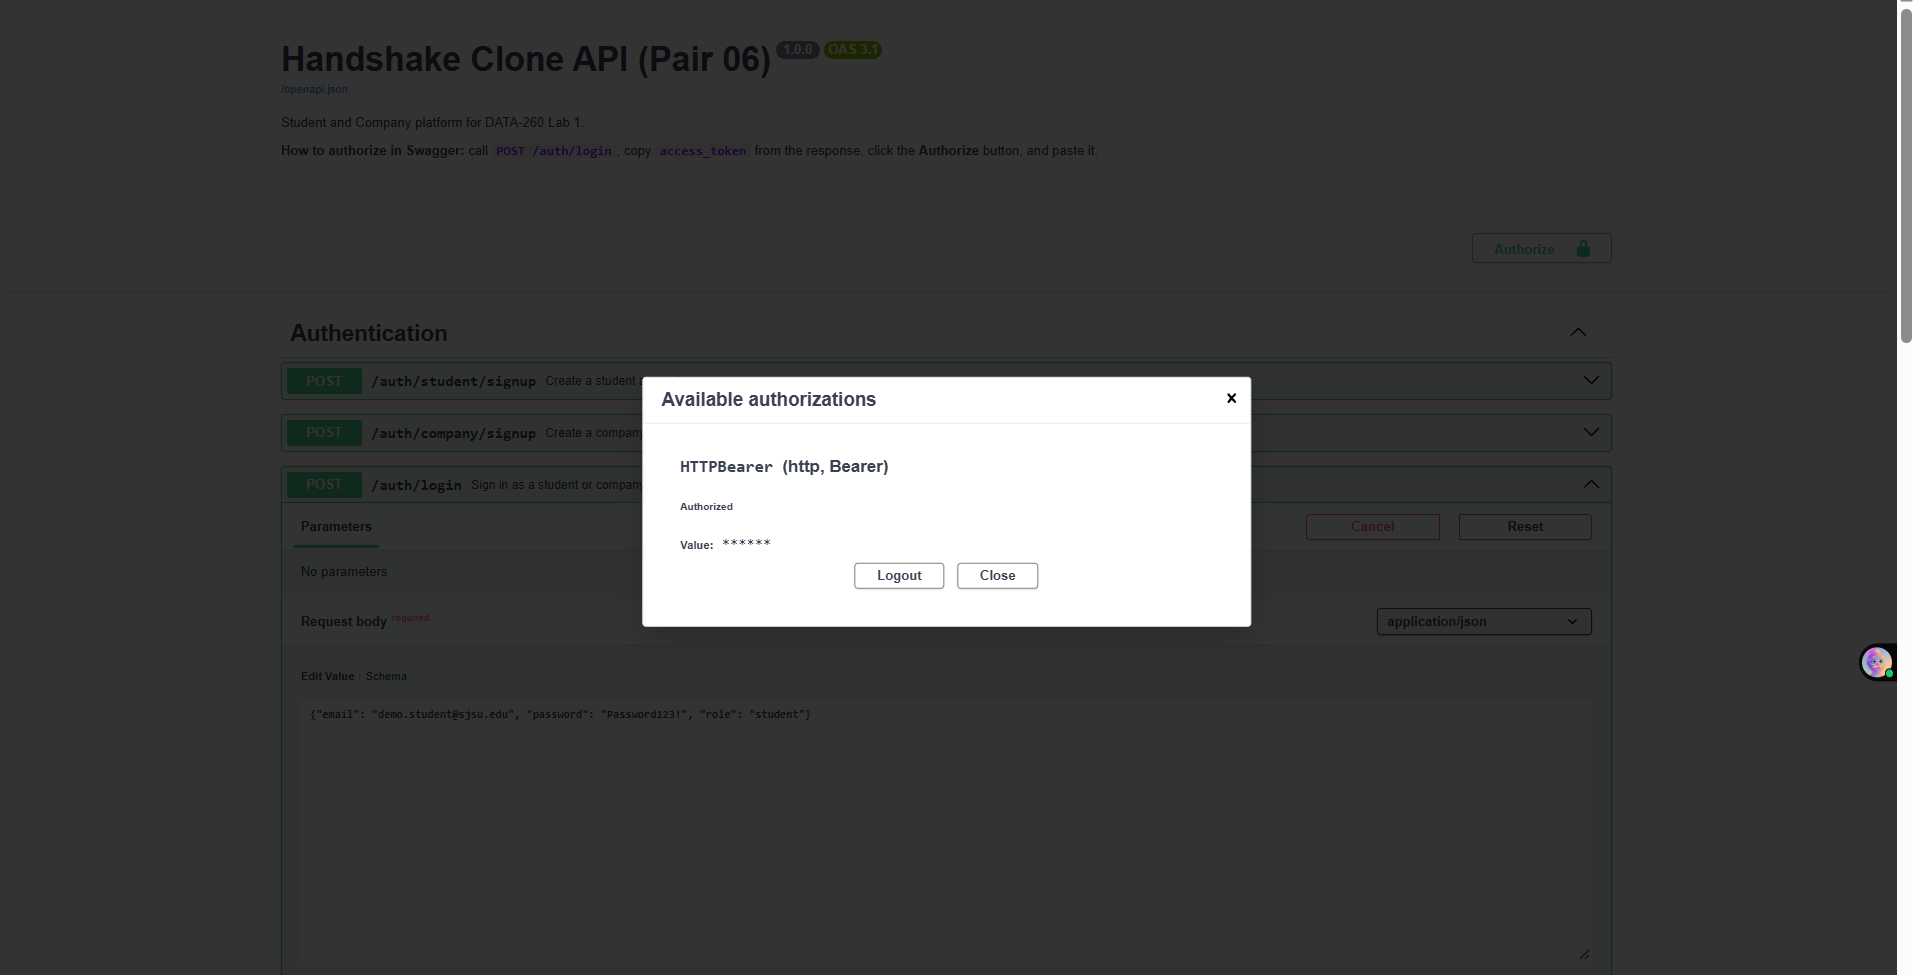
\includegraphics[width=\linewidth,height=0.42\textheight,keepaspectratio]{../screenshots/api_01_authorize_dialog.png}
\caption{Swagger Authorize dialog with the login request body (token hidden)}
\end{figure}

\begin{figure}[H]
\centering
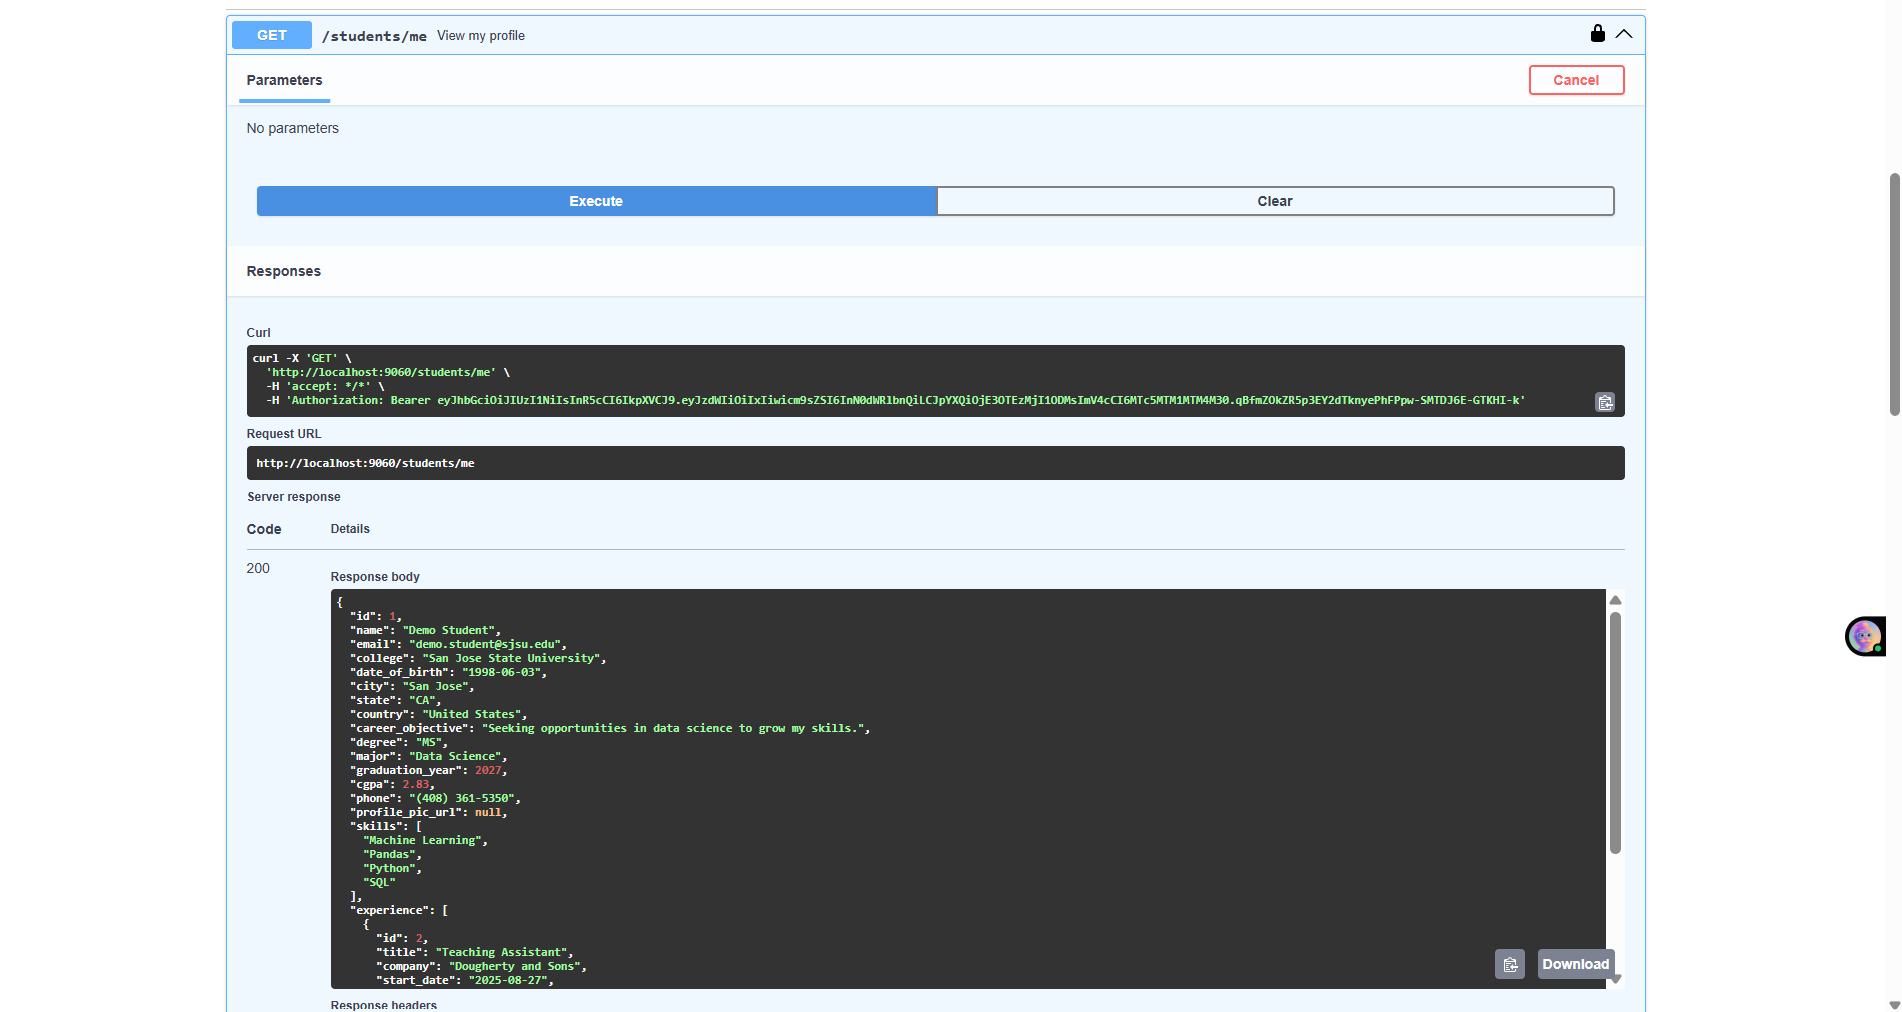
\includegraphics[width=\linewidth,height=0.42\textheight,keepaspectratio]{../screenshots/get_login_demo.png}
\caption{GET /students/me for the demo student (own view)}
\end{figure}

\begin{figure}[H]
\centering
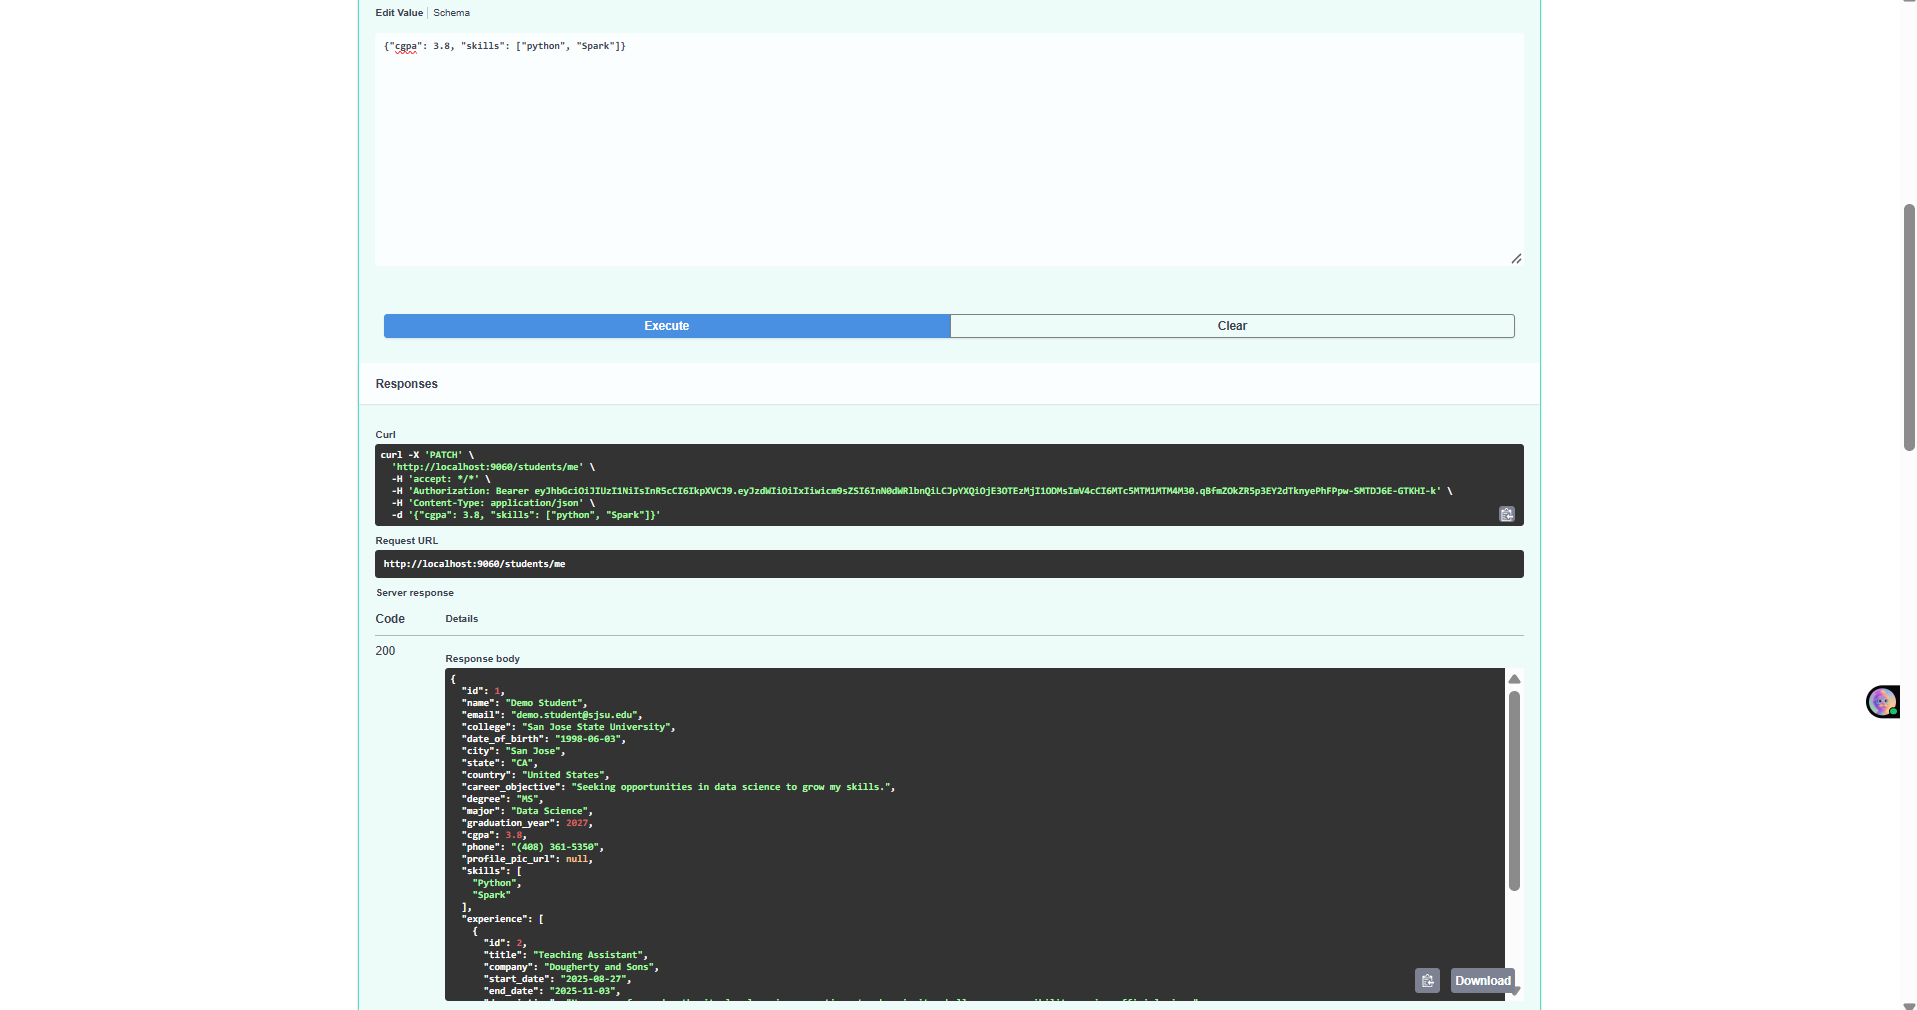
\includegraphics[width=\linewidth,height=0.42\textheight,keepaspectratio]{../screenshots/Update_demo.png}
\caption{PATCH /students/me changes GPA and skills}
\end{figure}

\begin{figure}[H]
\centering
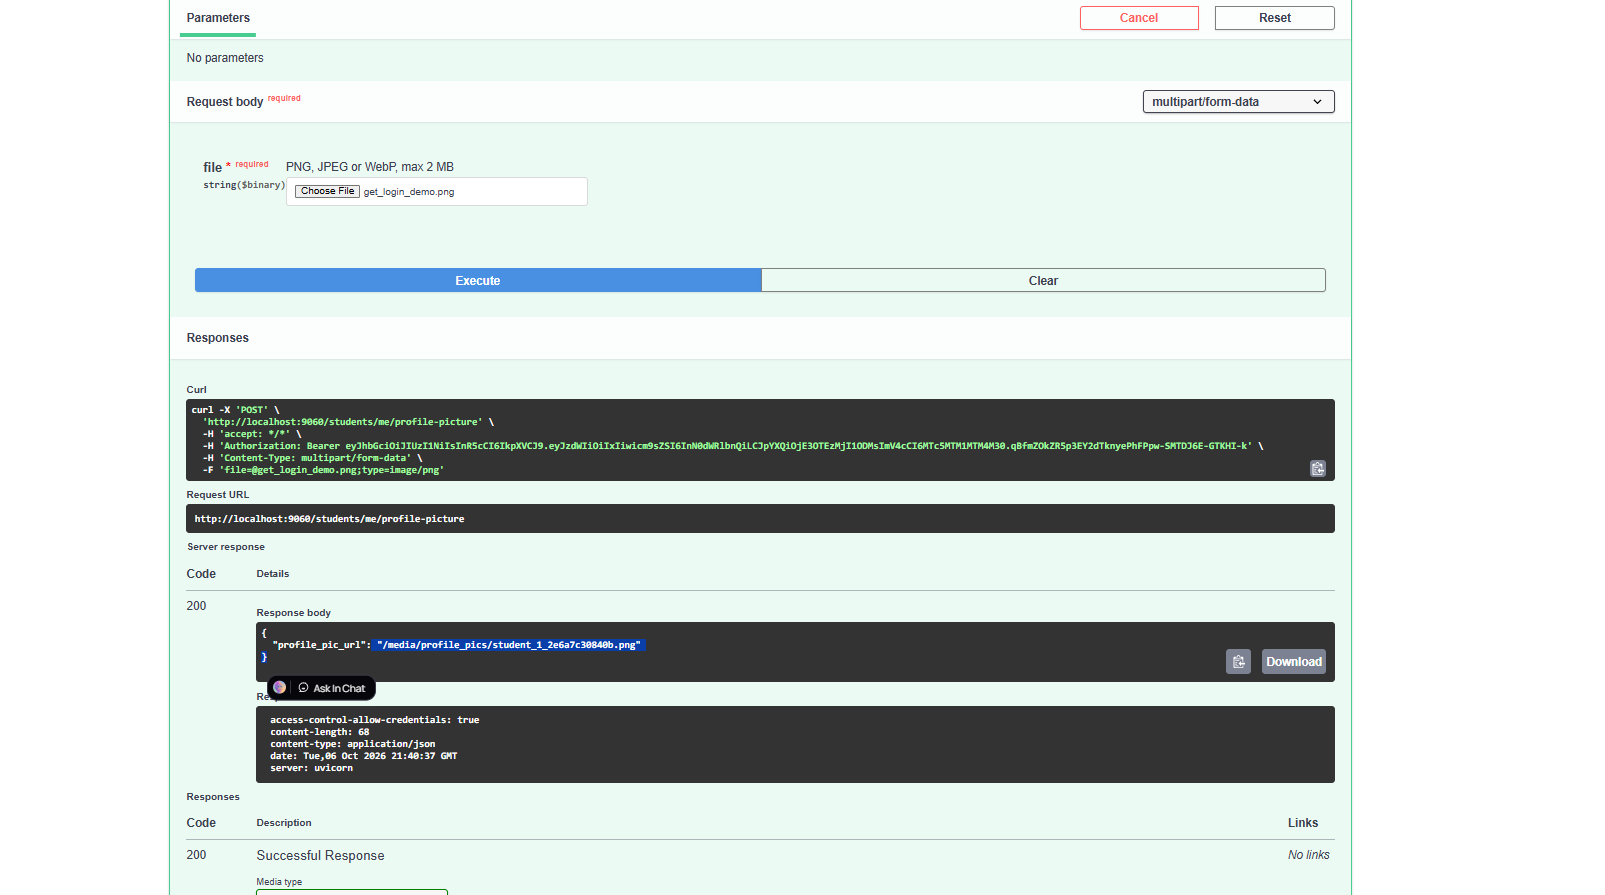
\includegraphics[width=\linewidth,height=0.42\textheight,keepaspectratio]{../screenshots/Profil_pic_demo.png}
\caption{POST /students/me/profile-picture returns the public picture URL}
\end{figure}

\begin{figure}[H]
\centering
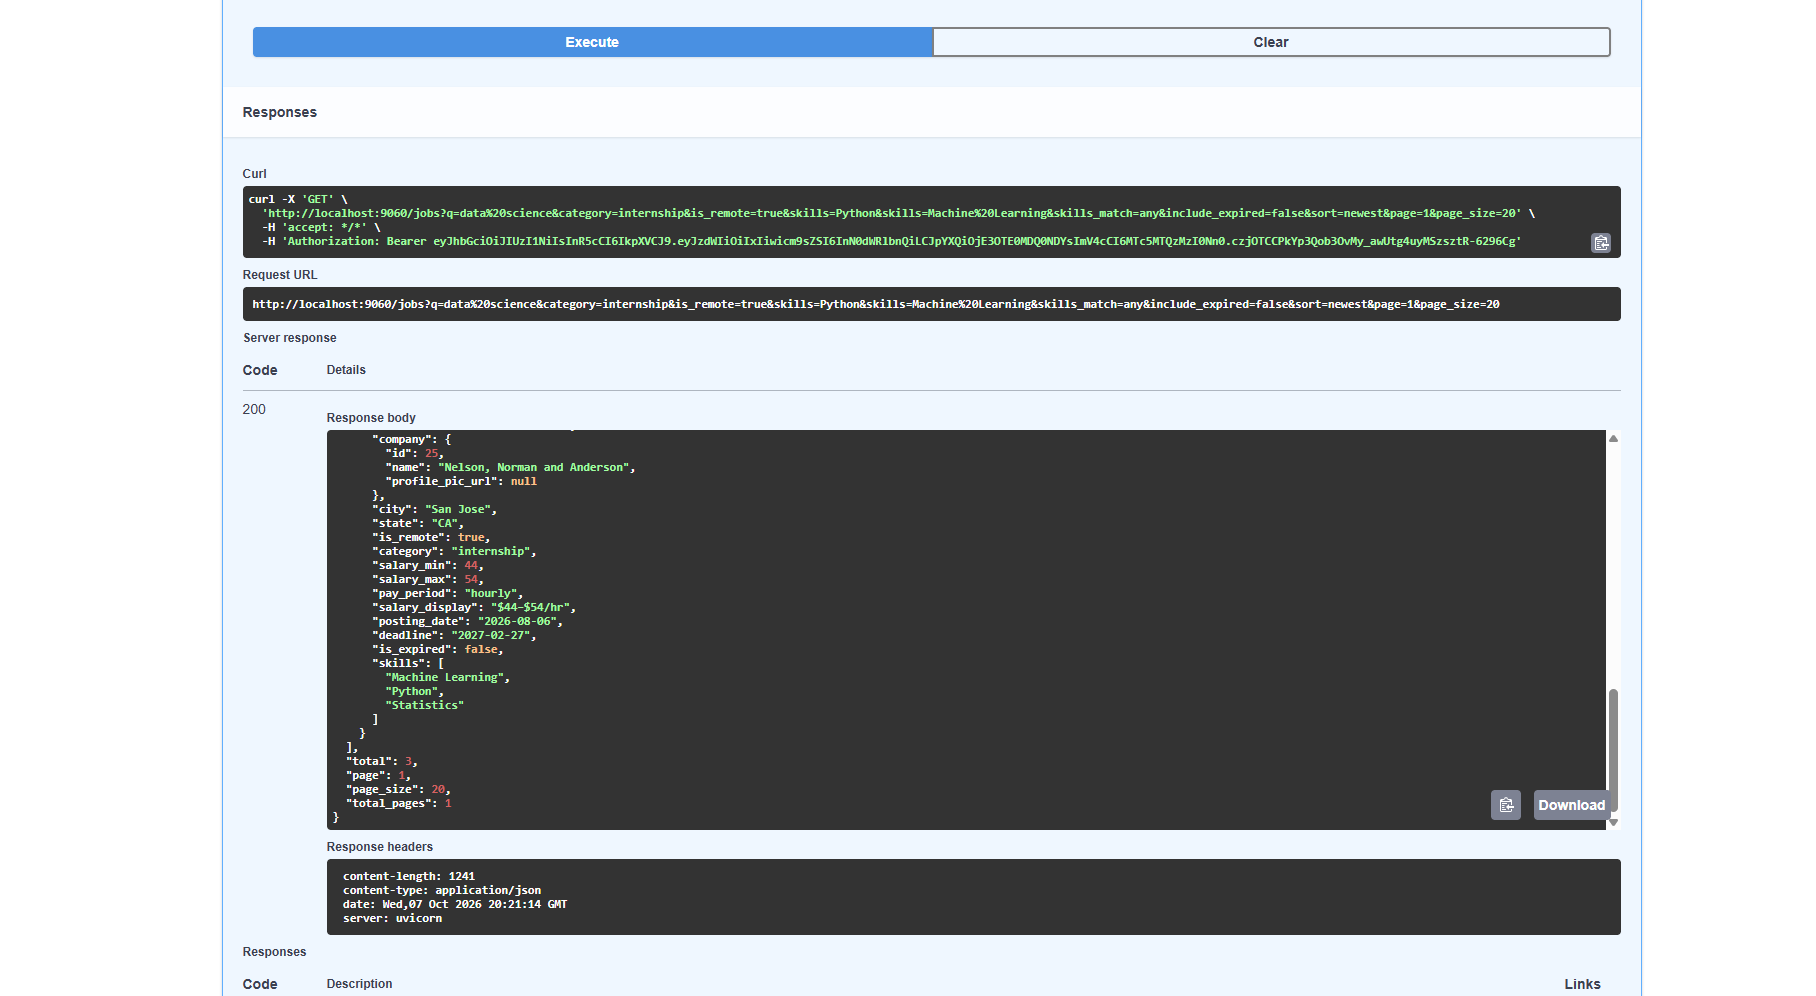
\includegraphics[width=\linewidth,height=0.42\textheight,keepaspectratio]{../screenshots/api_02_jobs_filters_200.png}
\caption{GET /jobs with title, category, remote and skills filters}
\end{figure}

\begin{figure}[H]
\centering
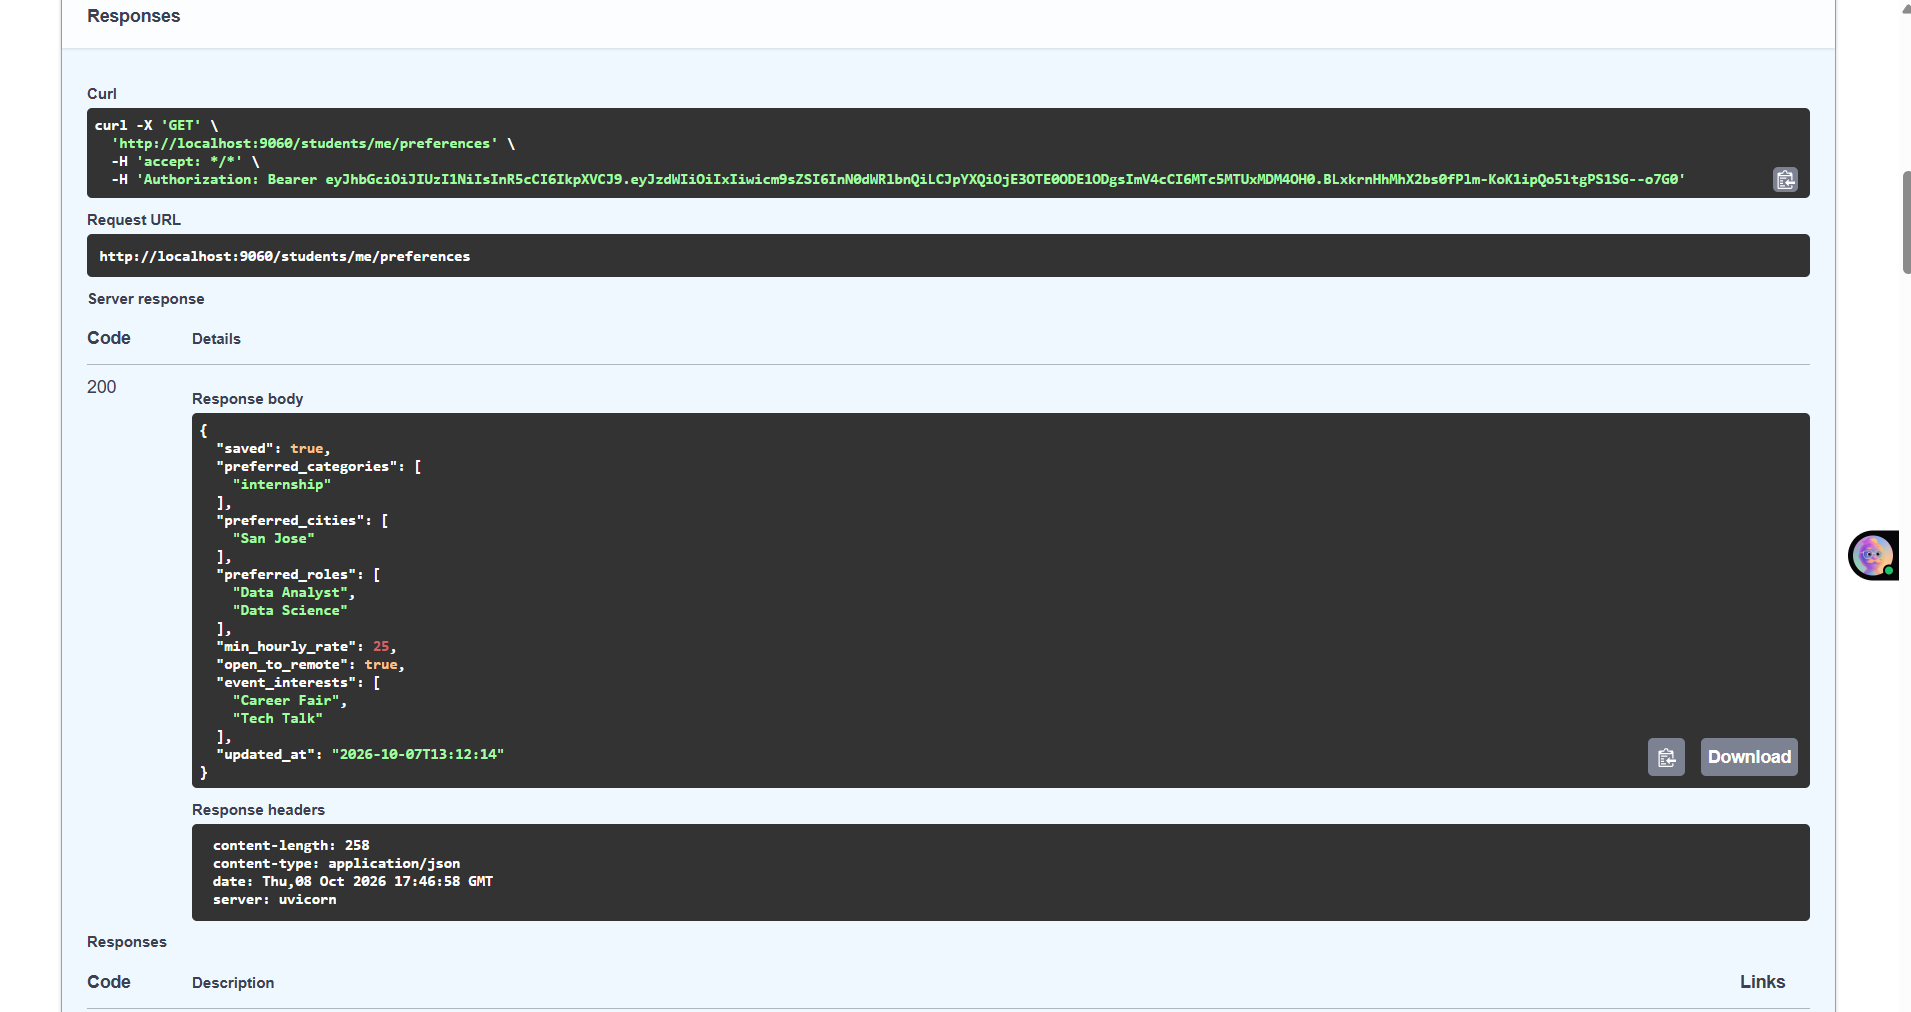
\includegraphics[width=\linewidth,height=0.42\textheight,keepaspectratio]{../screenshots/api_03_student_preferences_200.png}
\caption{GET /students/me/preferences}
\end{figure}

\subsection*{5.3 -- Swagger UI: applications and events (student token)}

\begin{figure}[H]
\centering
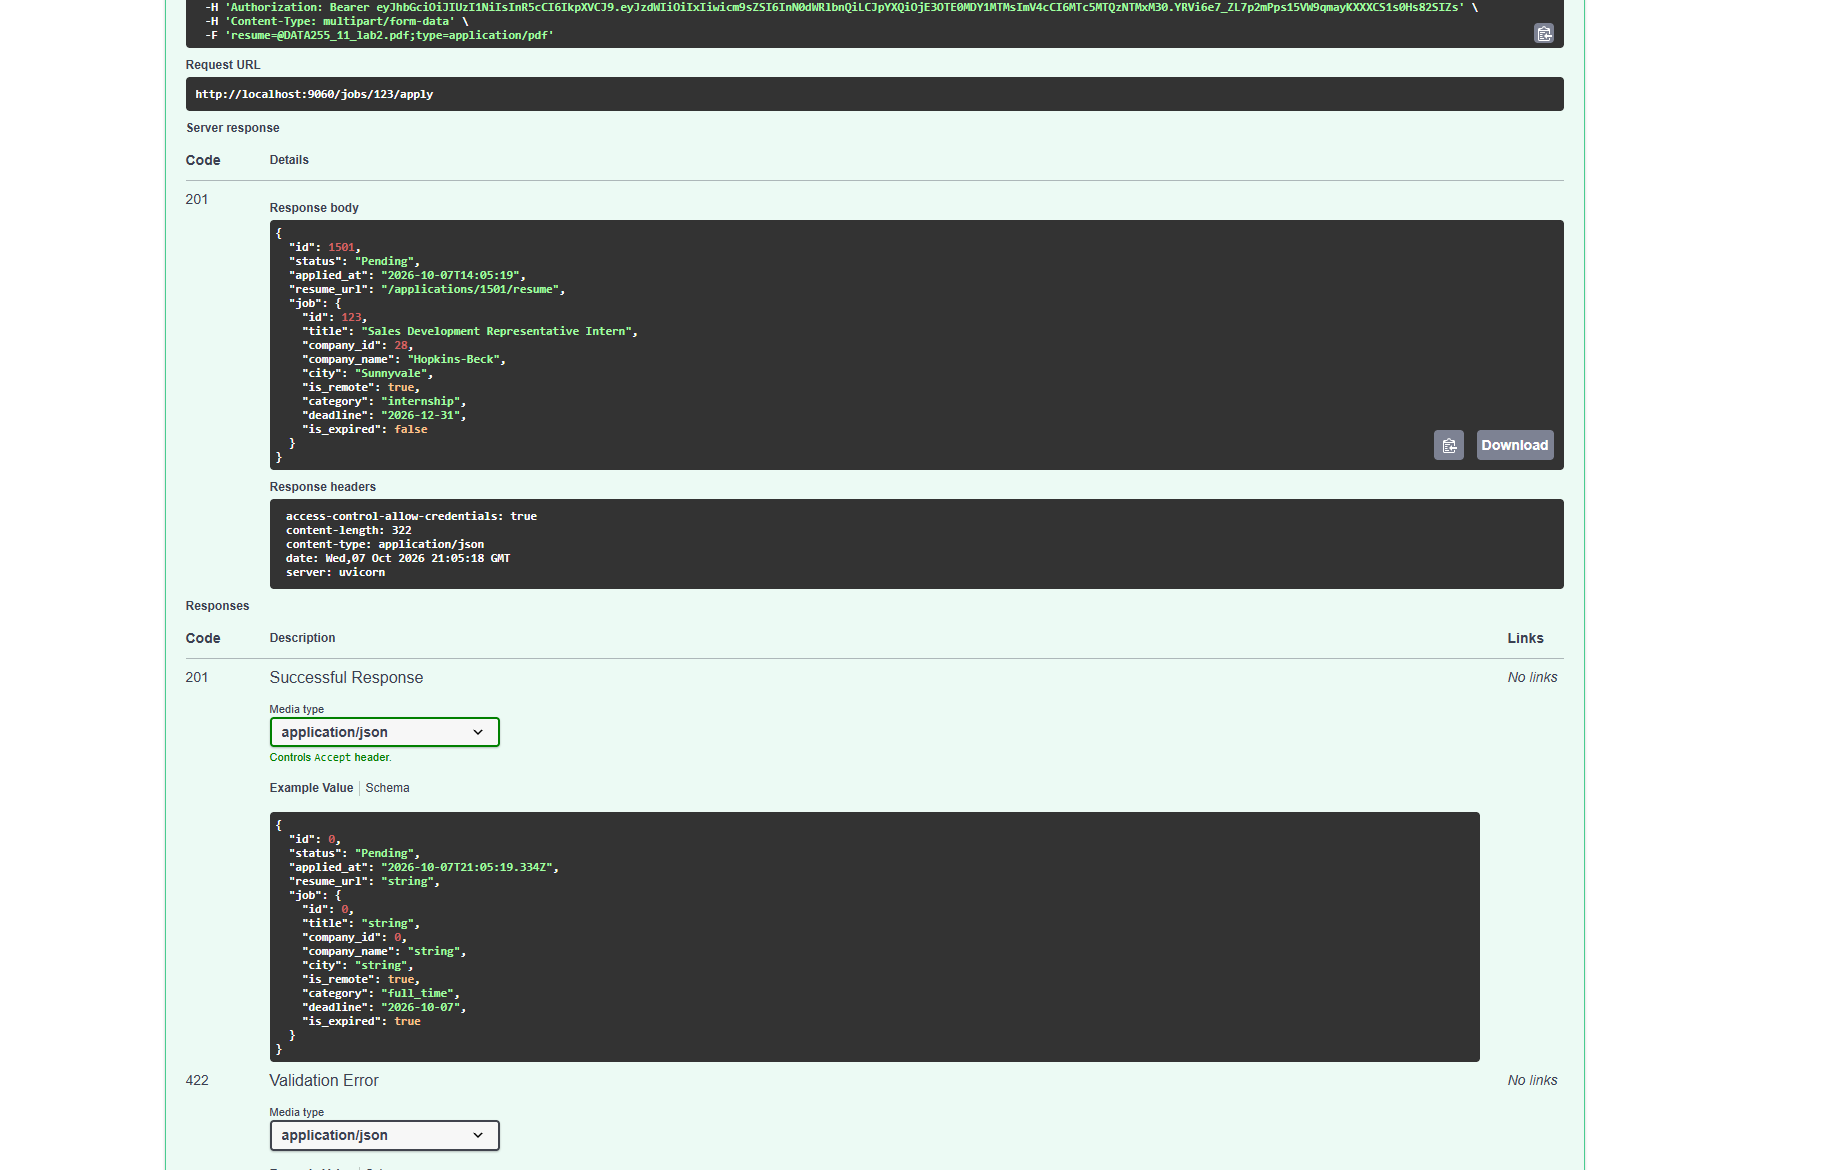
\includegraphics[width=\linewidth,height=0.42\textheight,keepaspectratio]{../screenshots/api_04_student_apply_201.png}
\caption{POST /jobs/123/apply with a PDF resume returns 201}
\end{figure}

\begin{figure}[H]
\centering
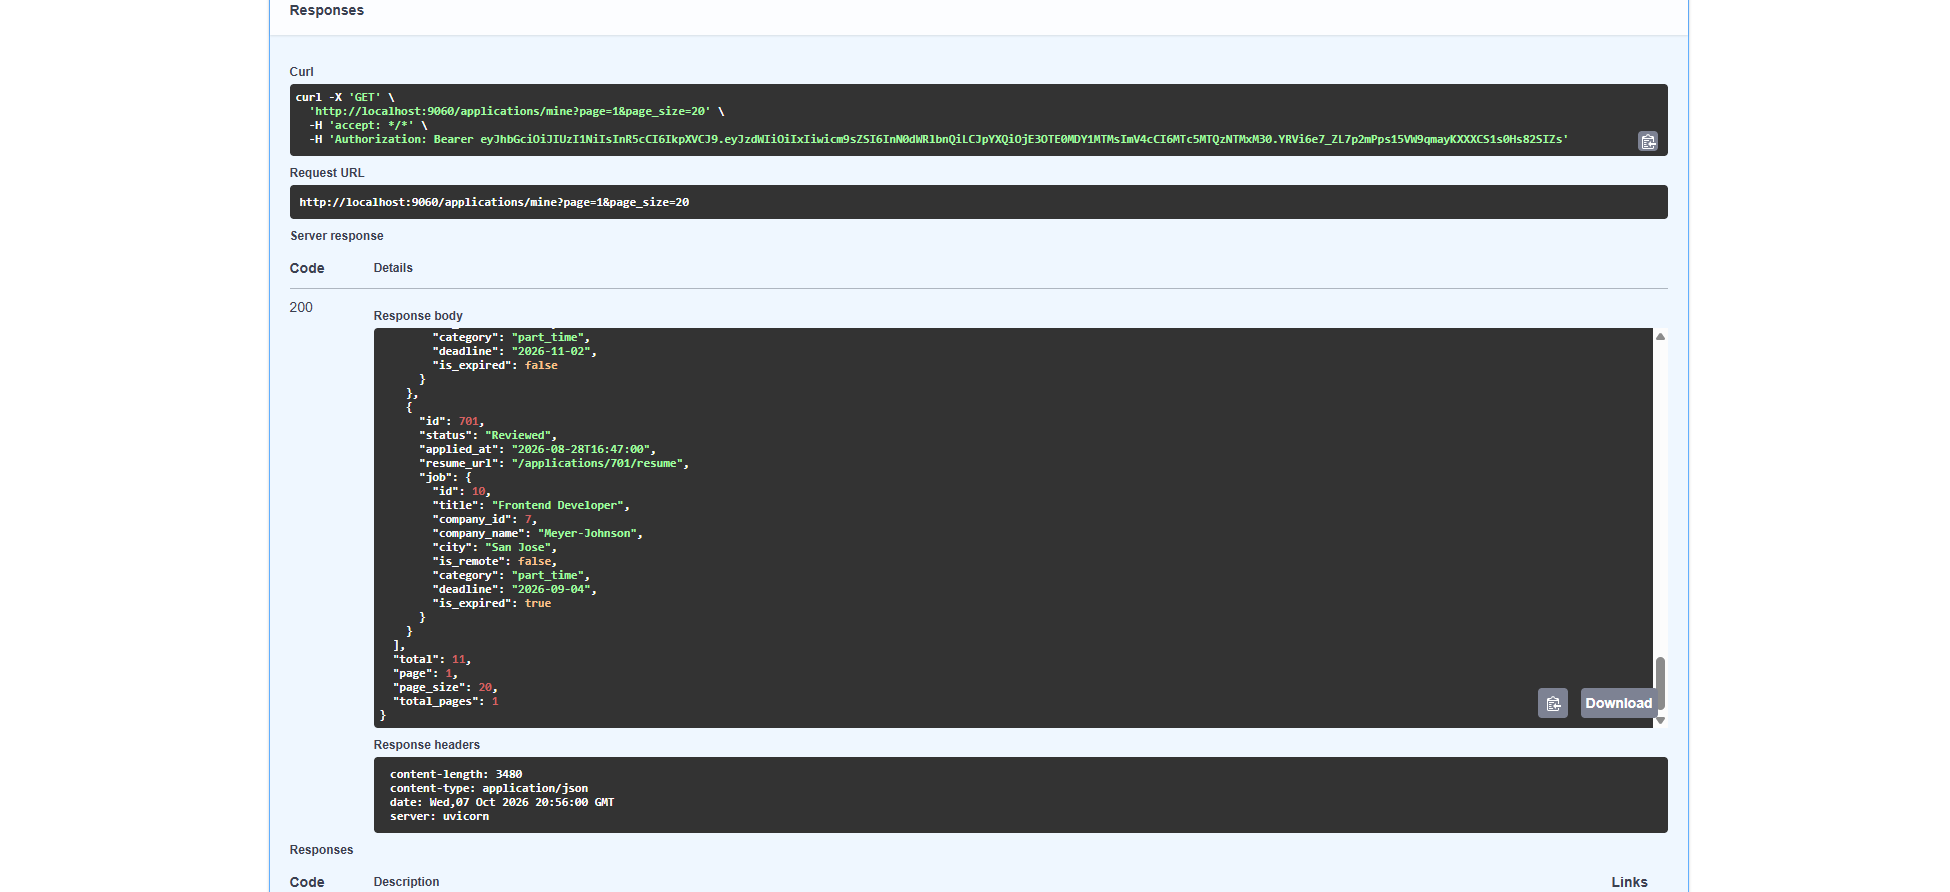
\includegraphics[width=\linewidth,height=0.42\textheight,keepaspectratio]{../screenshots/api_05_student_my_applications_200.png}
\caption{GET /applications/mine}
\end{figure}

\begin{figure}[H]
\centering
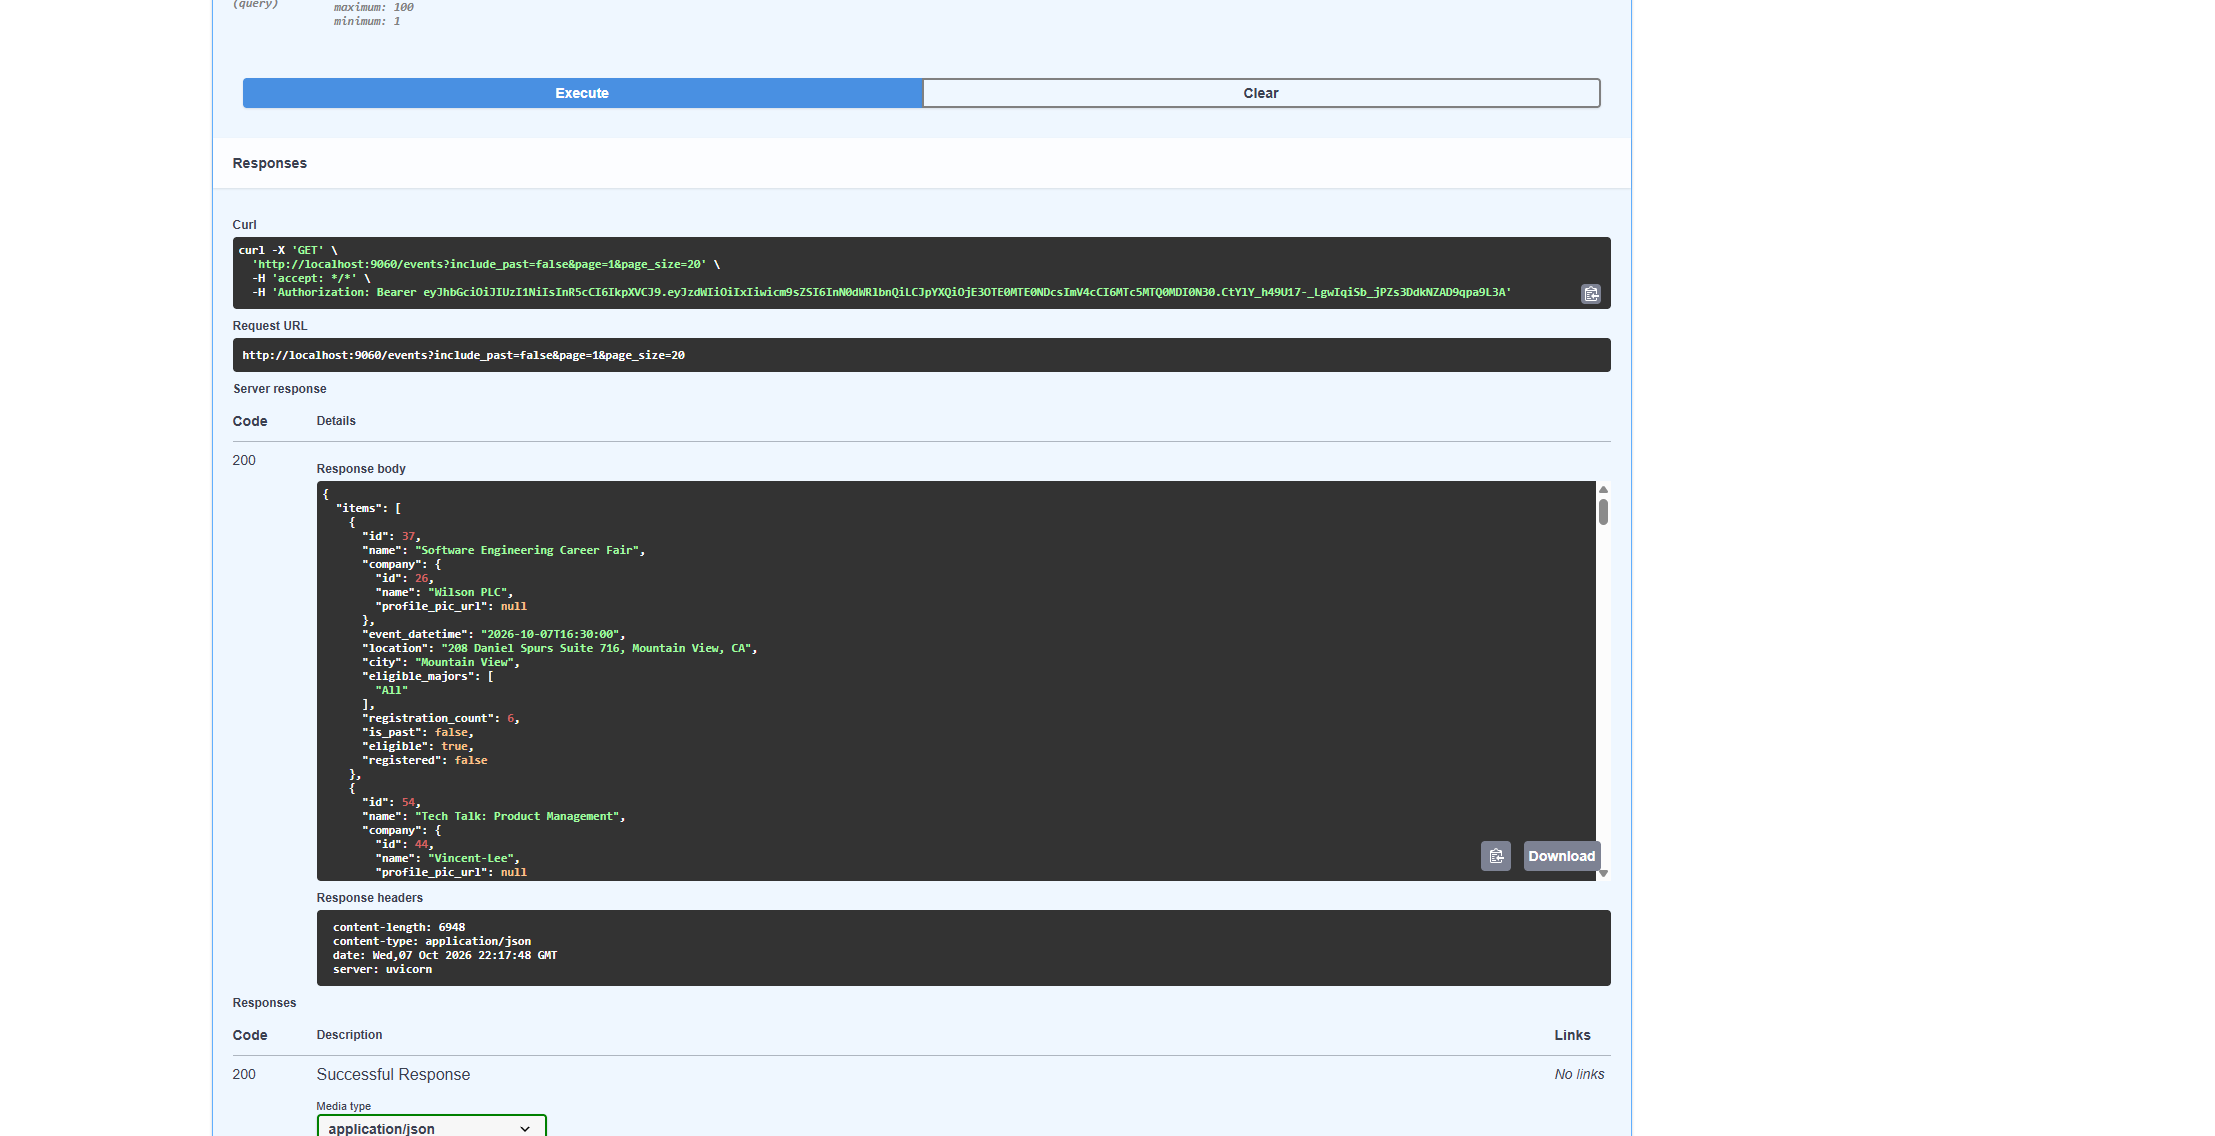
\includegraphics[width=\linewidth,height=0.42\textheight,keepaspectratio]{../screenshots/api_06_student_events_200.png}
\caption{GET /events (upcoming)}
\end{figure}

\begin{figure}[H]
\centering
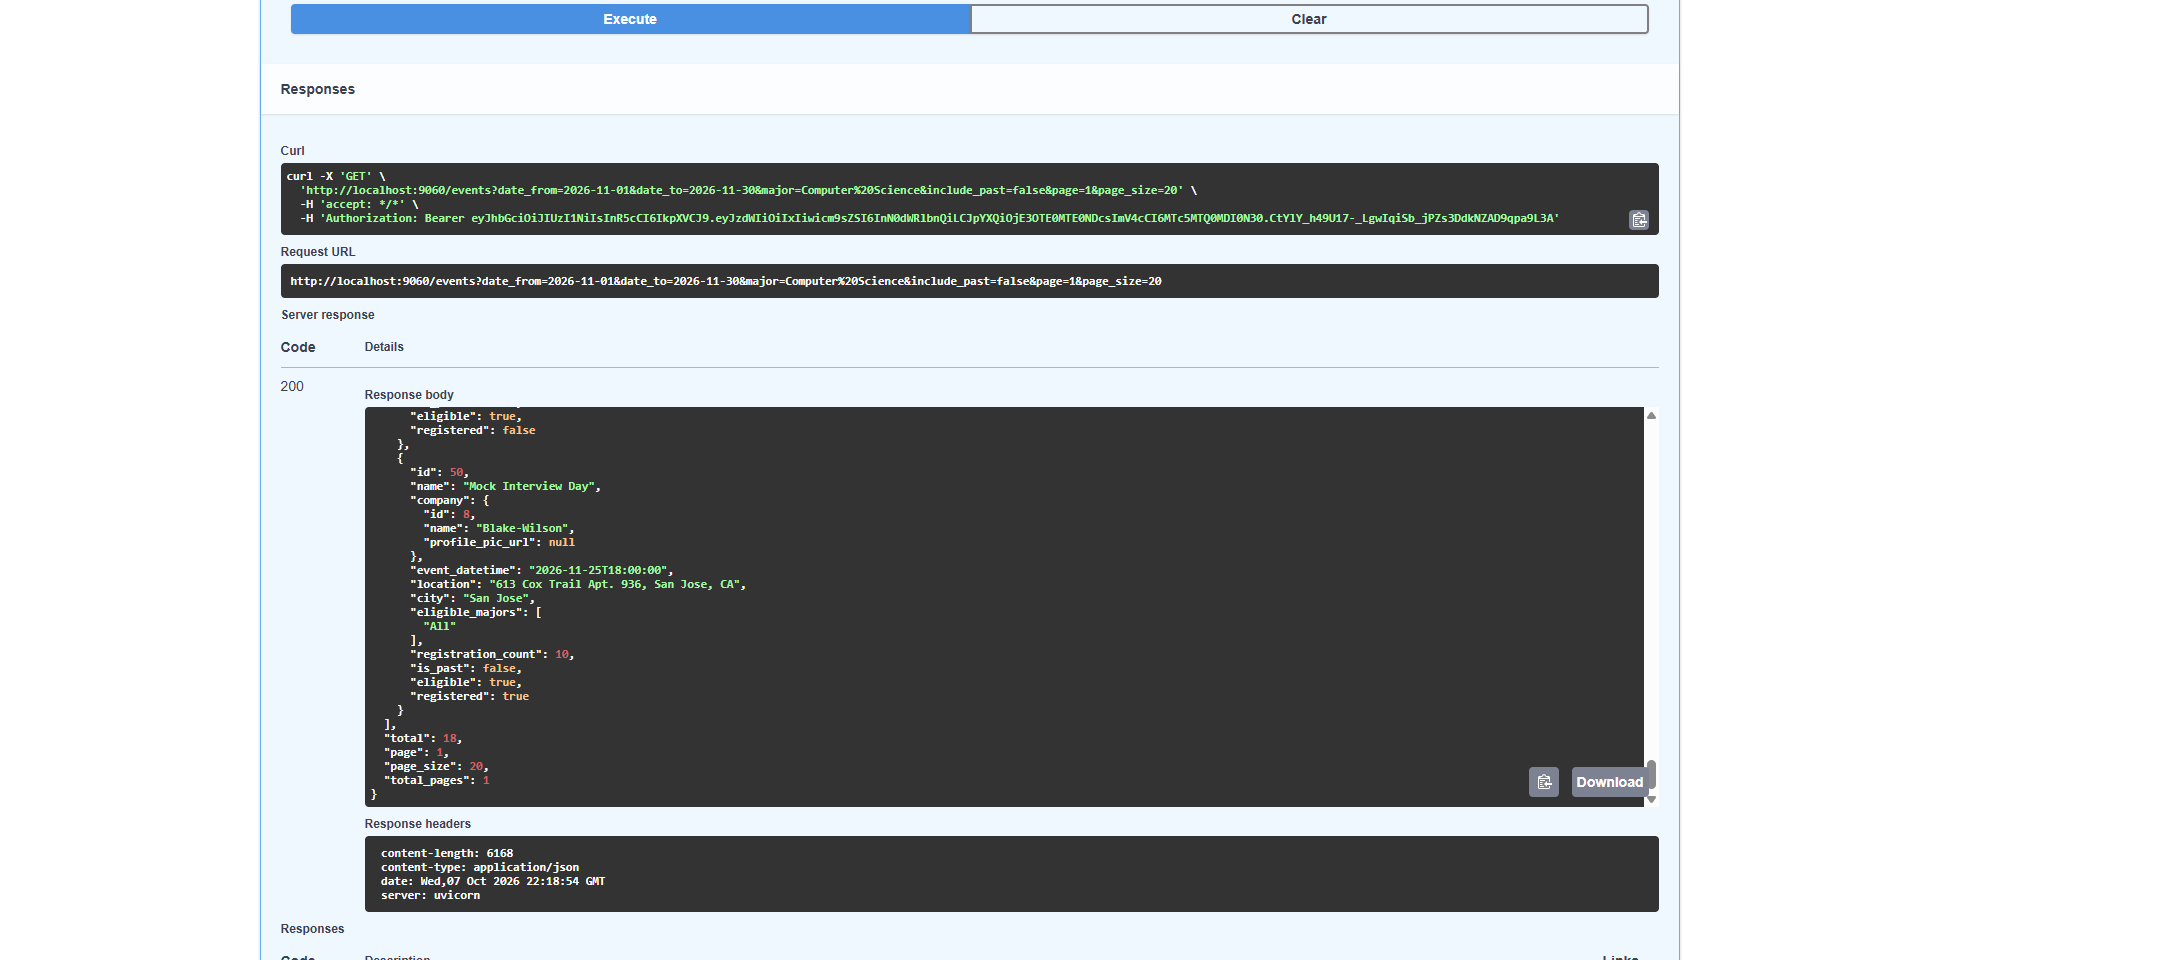
\includegraphics[width=\linewidth,height=0.42\textheight,keepaspectratio]{../screenshots/api_07_student_events_filtered_200.png}
\caption{GET /events filtered by date range and major}
\end{figure}

\begin{figure}[H]
\centering
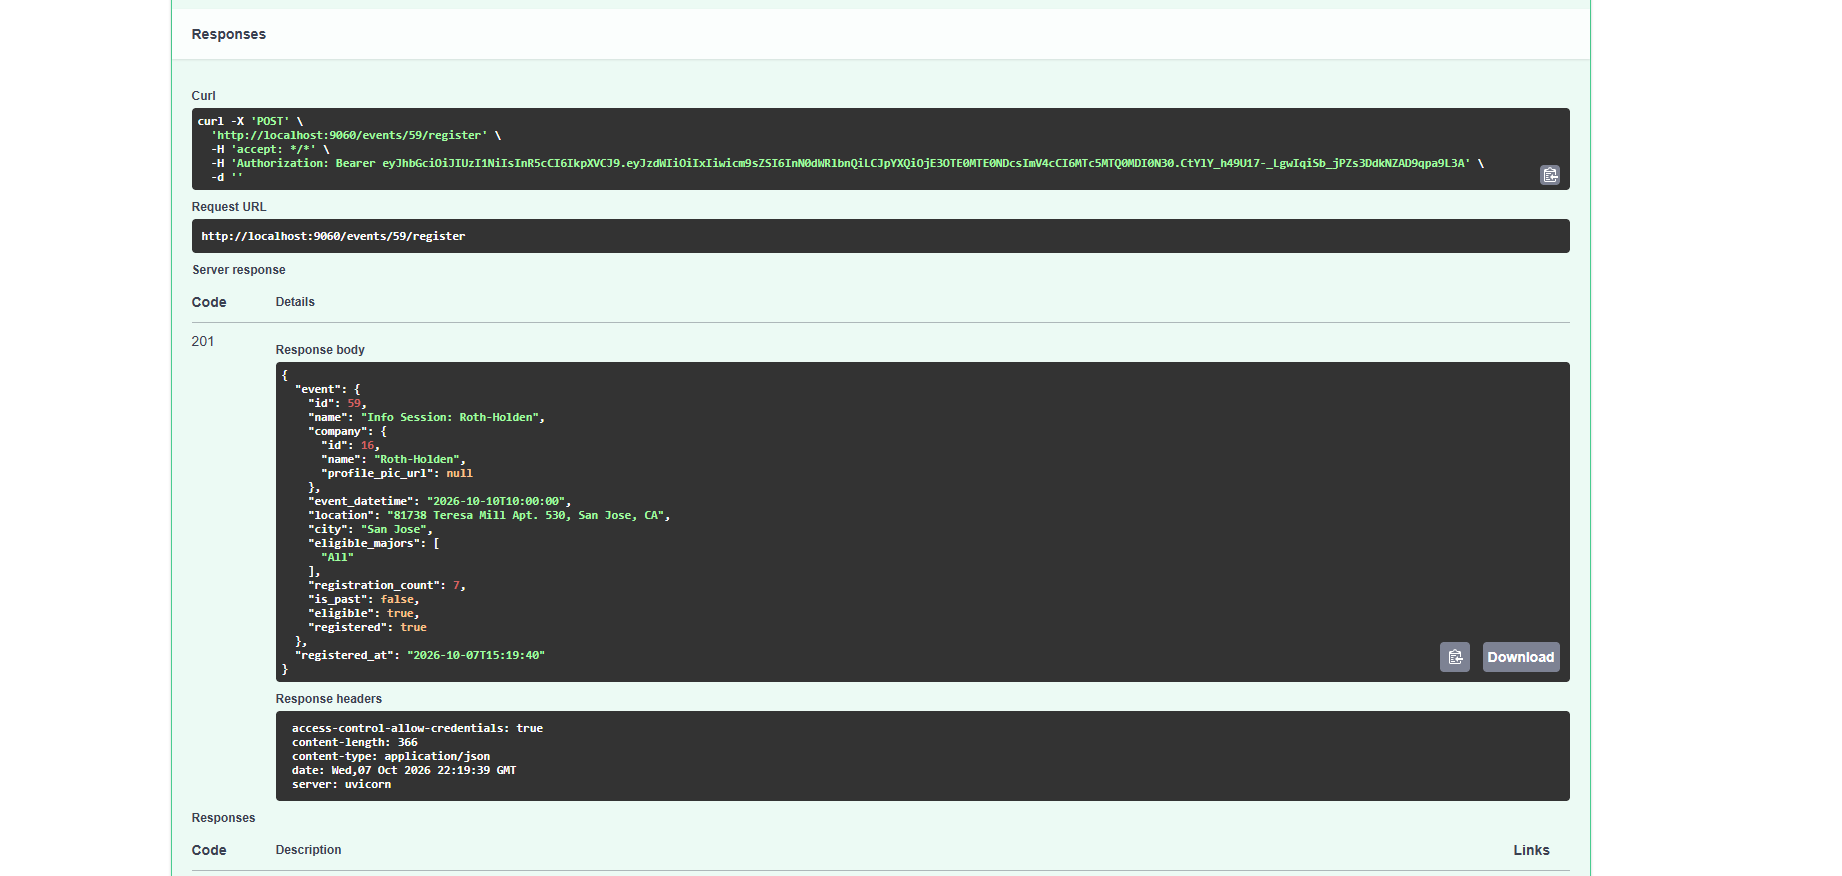
\includegraphics[width=\linewidth,height=0.42\textheight,keepaspectratio]{../screenshots/api_08_event_register_201.png}
\caption{POST /events/59/register returns 201}
\end{figure}

\begin{figure}[H]
\centering
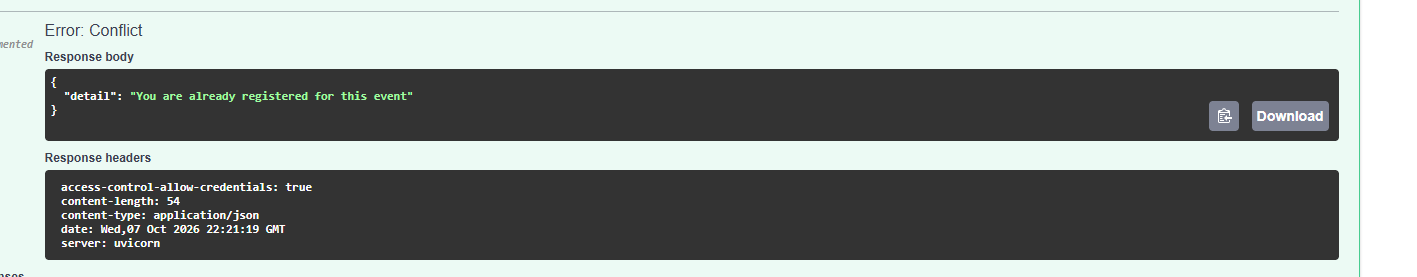
\includegraphics[width=\linewidth,height=0.42\textheight,keepaspectratio]{../screenshots/api_09_event_register_409_duplicate.png}
\caption{Registering again returns 409}
\end{figure}

\begin{figure}[H]
\centering
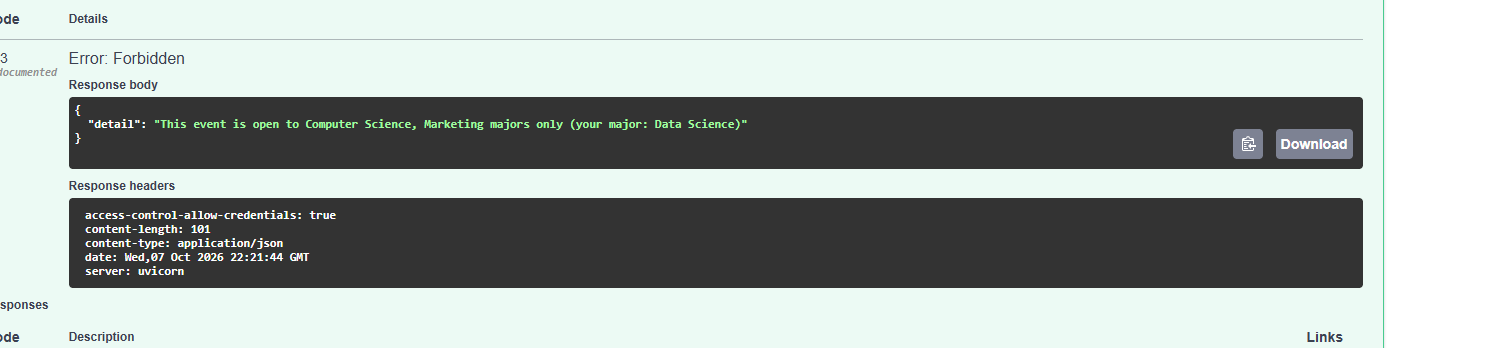
\includegraphics[width=\linewidth,height=0.42\textheight,keepaspectratio]{../screenshots/api_10_event_register_403_major.png}
\caption{Registering for an event closed to the student's major returns 403}
\end{figure}

\subsection*{5.4 -- Swagger UI: student directory, student token and company token}

\begin{figure}[H]
\centering
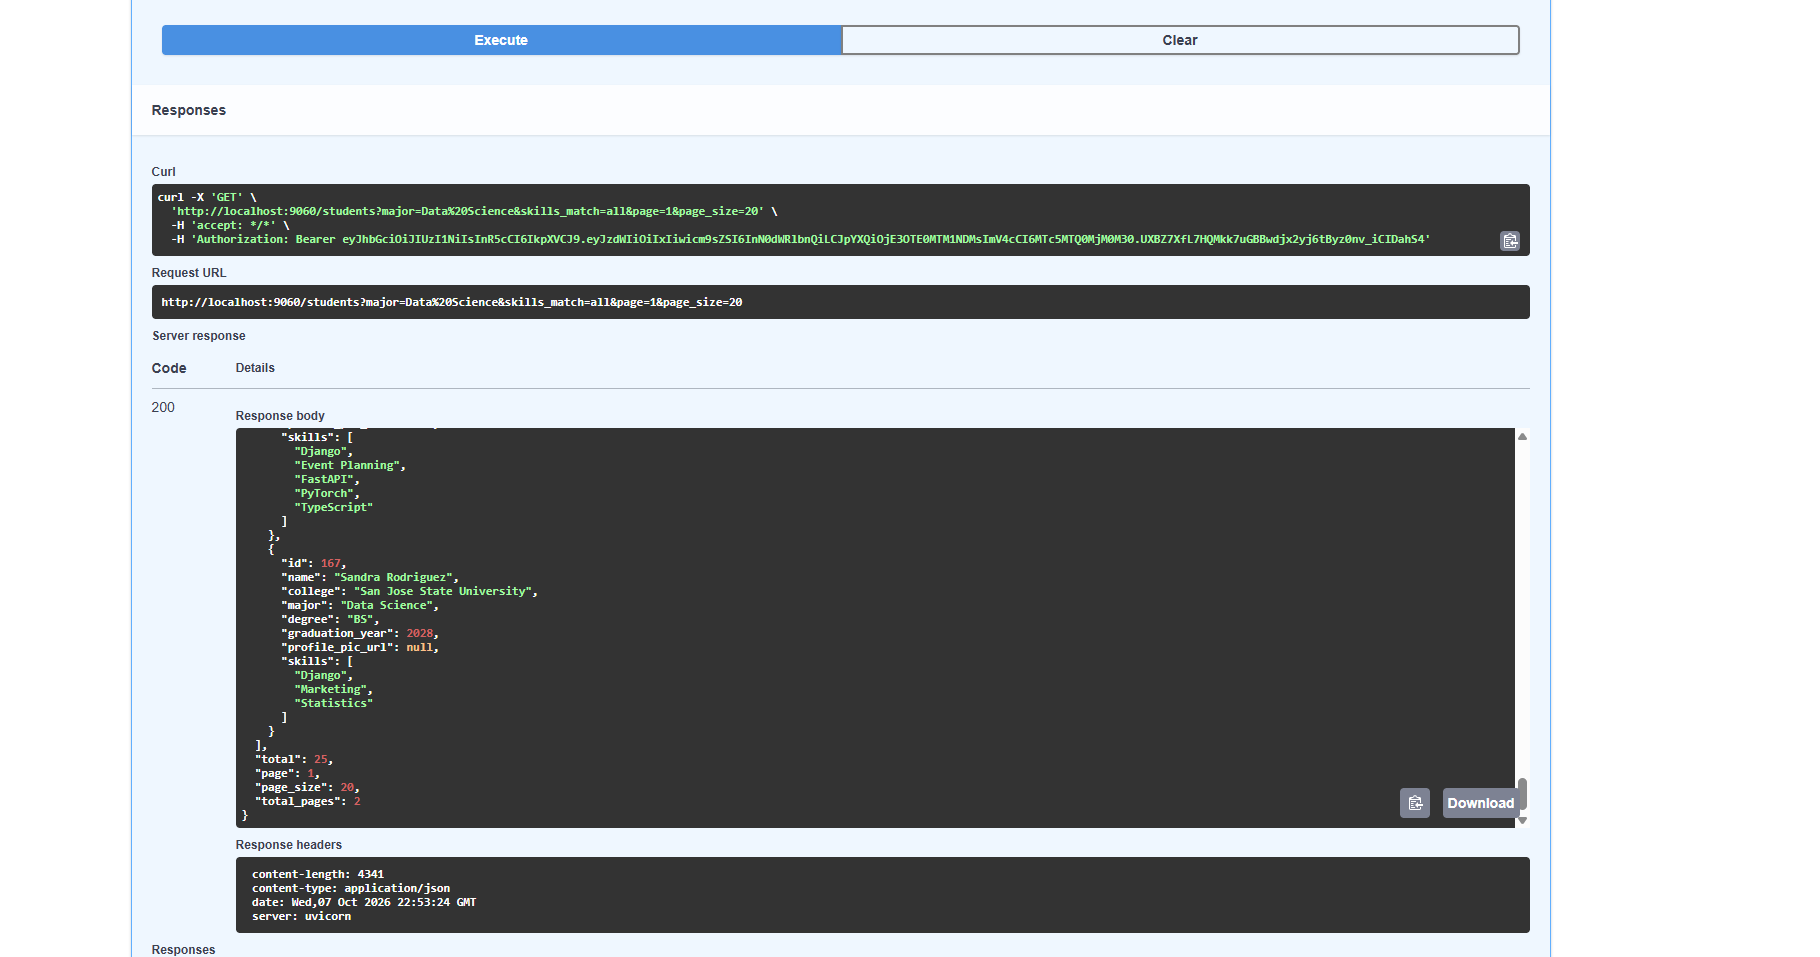
\includegraphics[width=\linewidth,height=0.42\textheight,keepaspectratio]{../screenshots/api_11_student_directory_peer_no_email.png}
\caption{GET /students as a student (peer view, no email)}
\end{figure}

\begin{figure}[H]
\centering
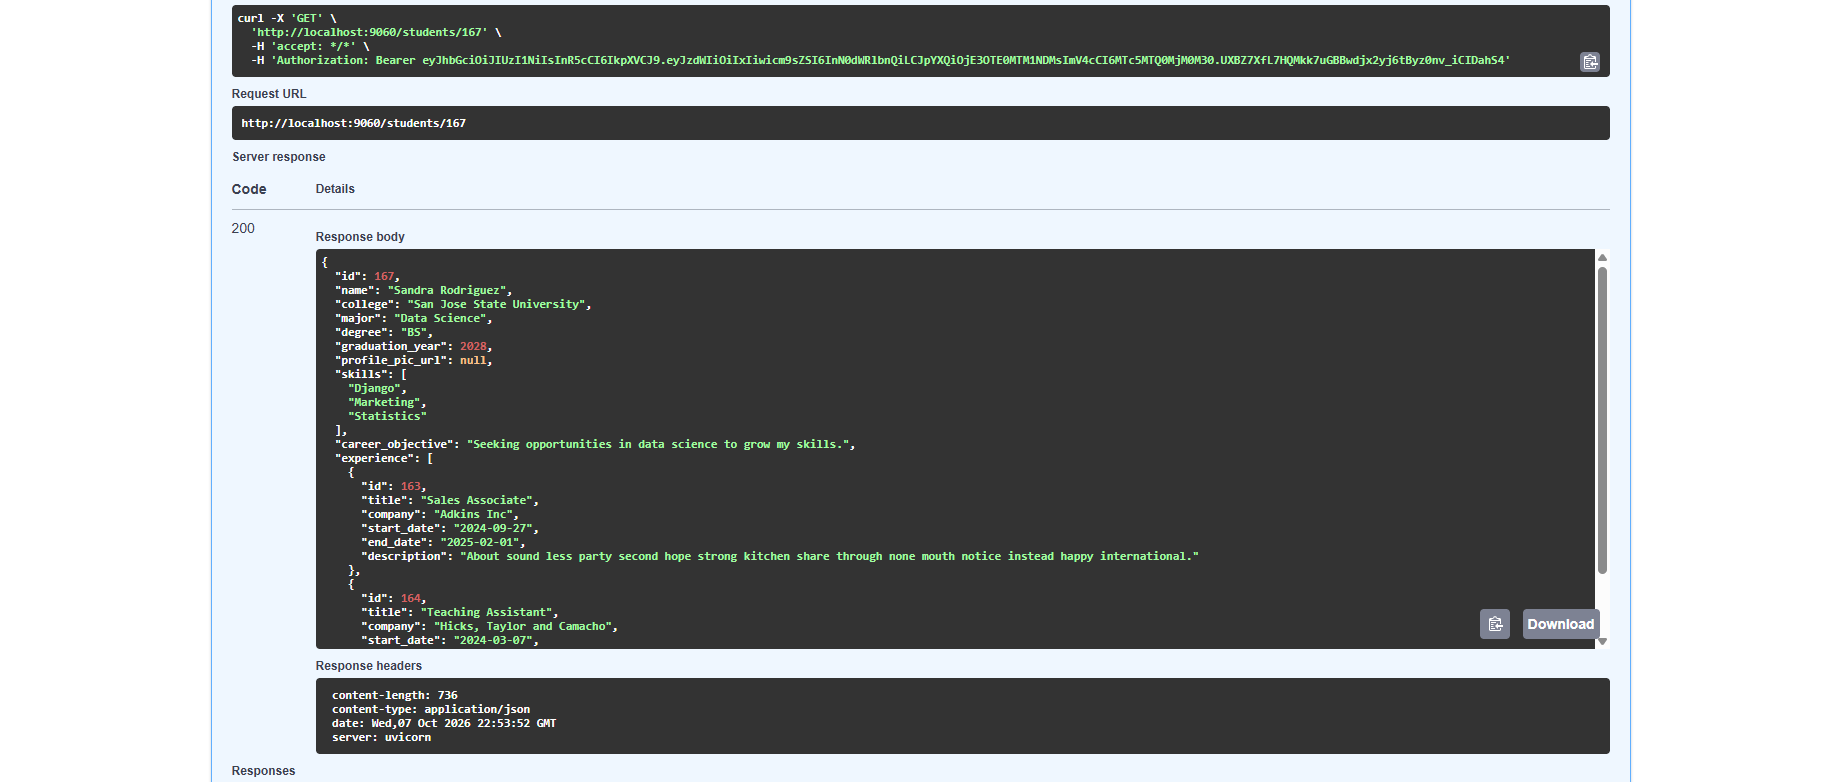
\includegraphics[width=\linewidth,height=0.42\textheight,keepaspectratio]{../screenshots/api_12_student_profile_peer_no_email.png}
\caption{GET /students/167 as a student (peer profile)}
\end{figure}

\begin{figure}[H]
\centering
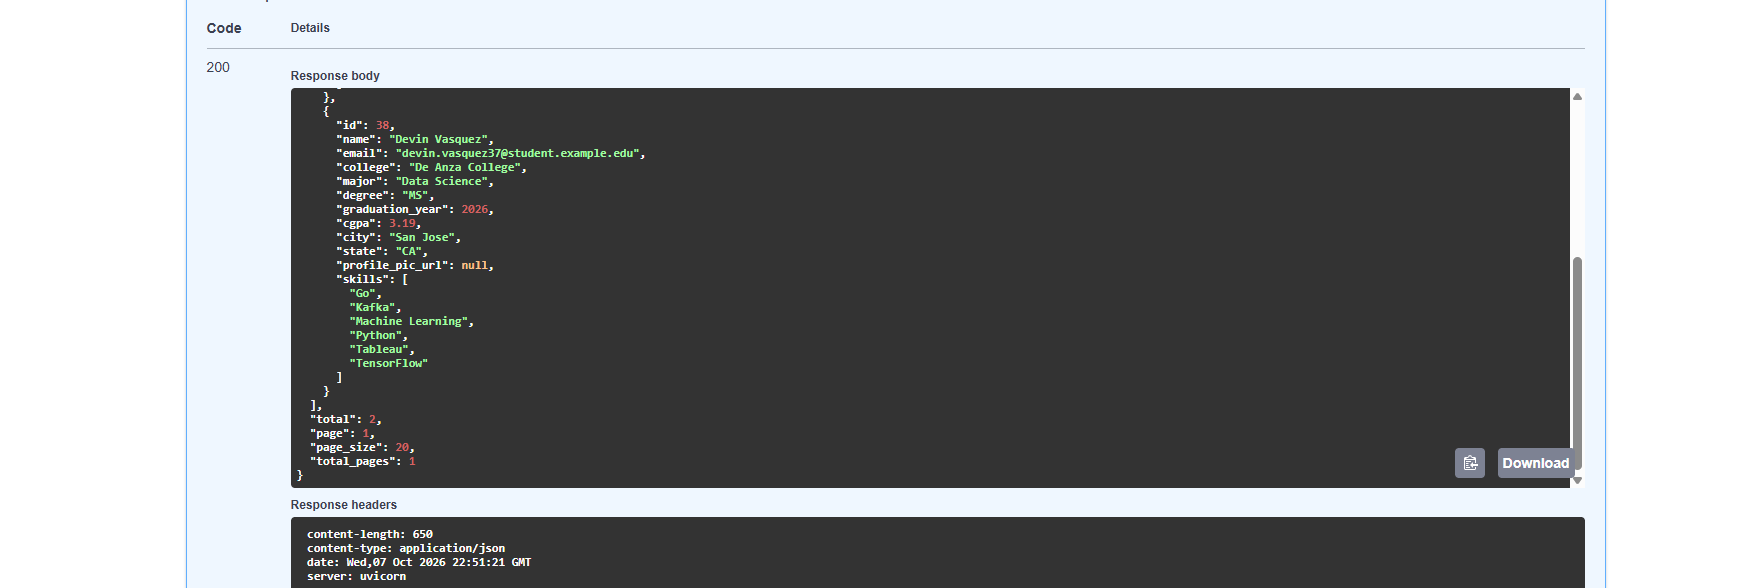
\includegraphics[width=\linewidth,height=0.42\textheight,keepaspectratio]{../screenshots/api_13_company_students_with_email.png}
\caption{GET /students as a company (email and GPA shown)}
\end{figure}

\begin{figure}[H]
\centering
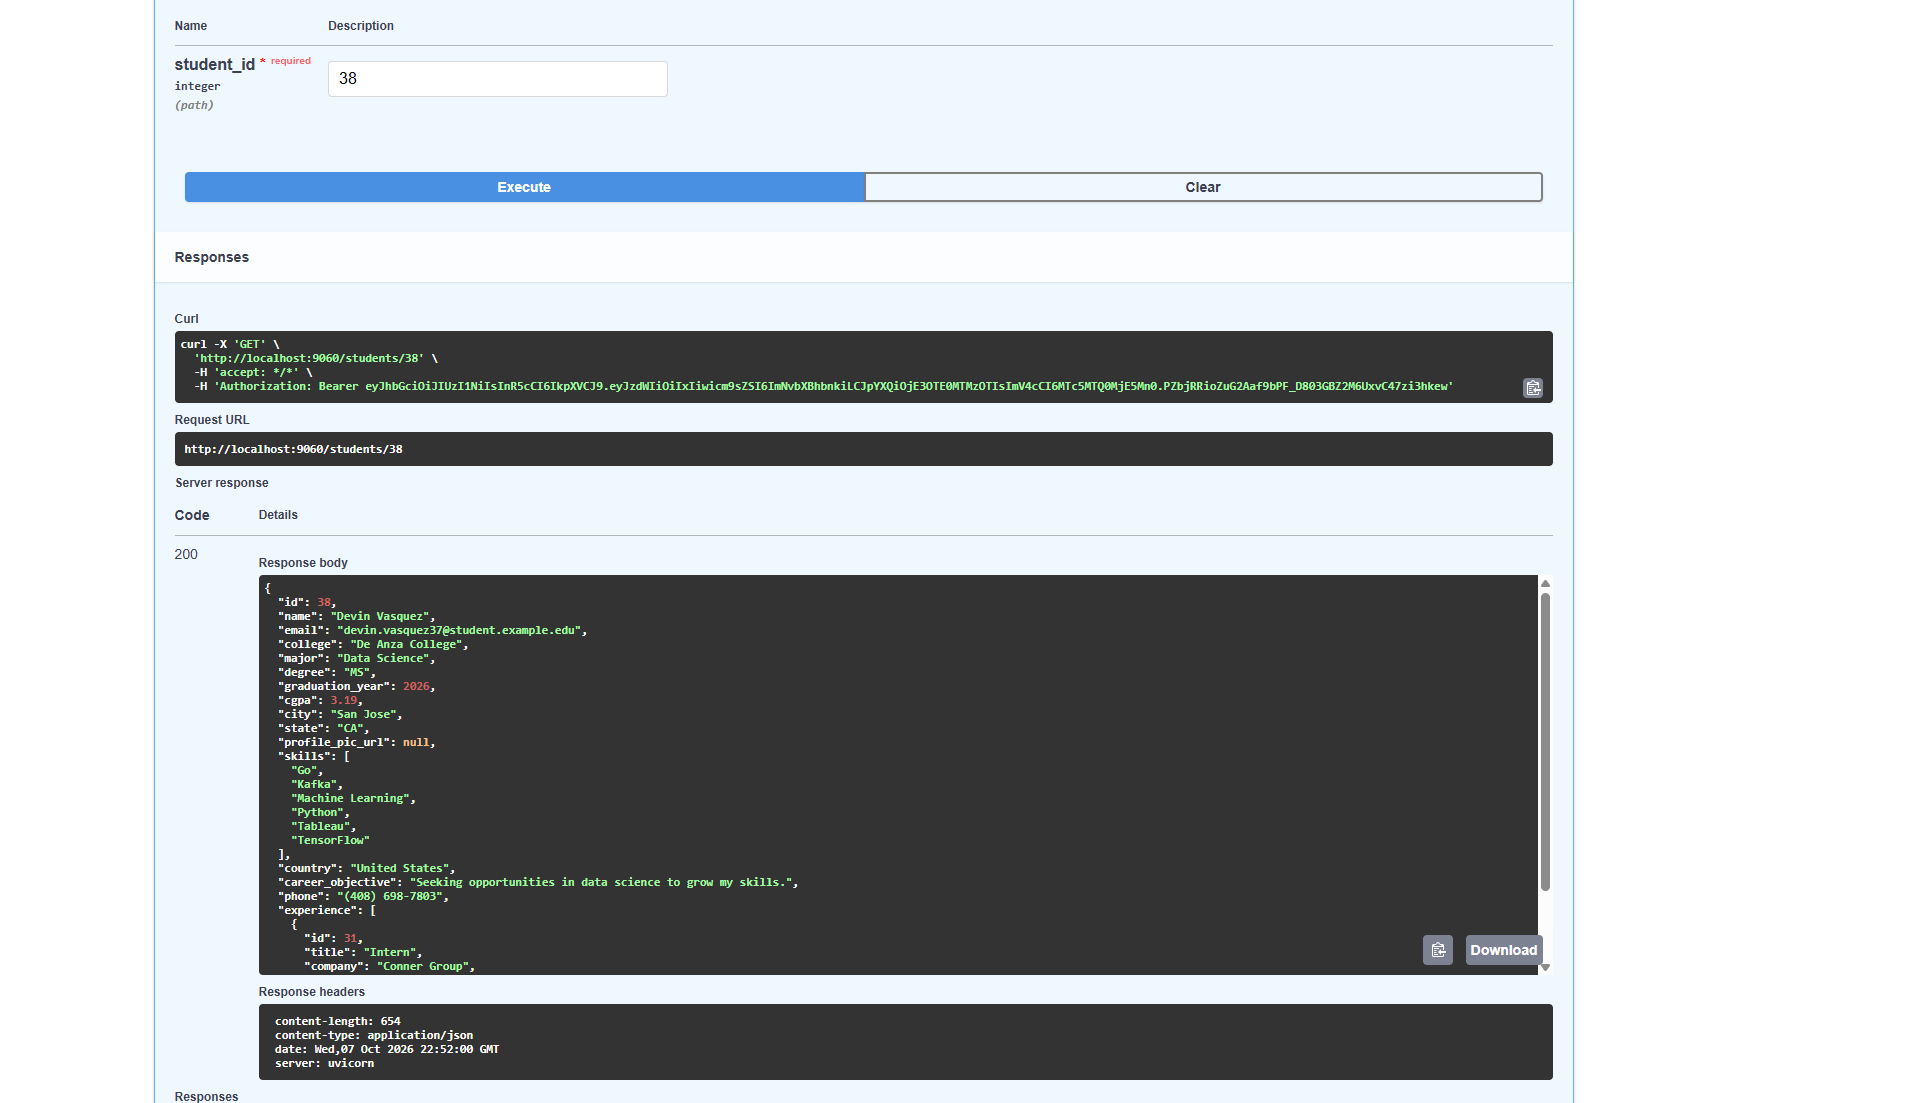
\includegraphics[width=\linewidth,height=0.42\textheight,keepaspectratio]{../screenshots/api_14_company_student_detail_with_email_phone.png}
\caption{GET /students/38 as a company (email, GPA and phone)}
\end{figure}

\subsection*{5.5 -- Swagger UI: company token}

\begin{figure}[H]
\centering
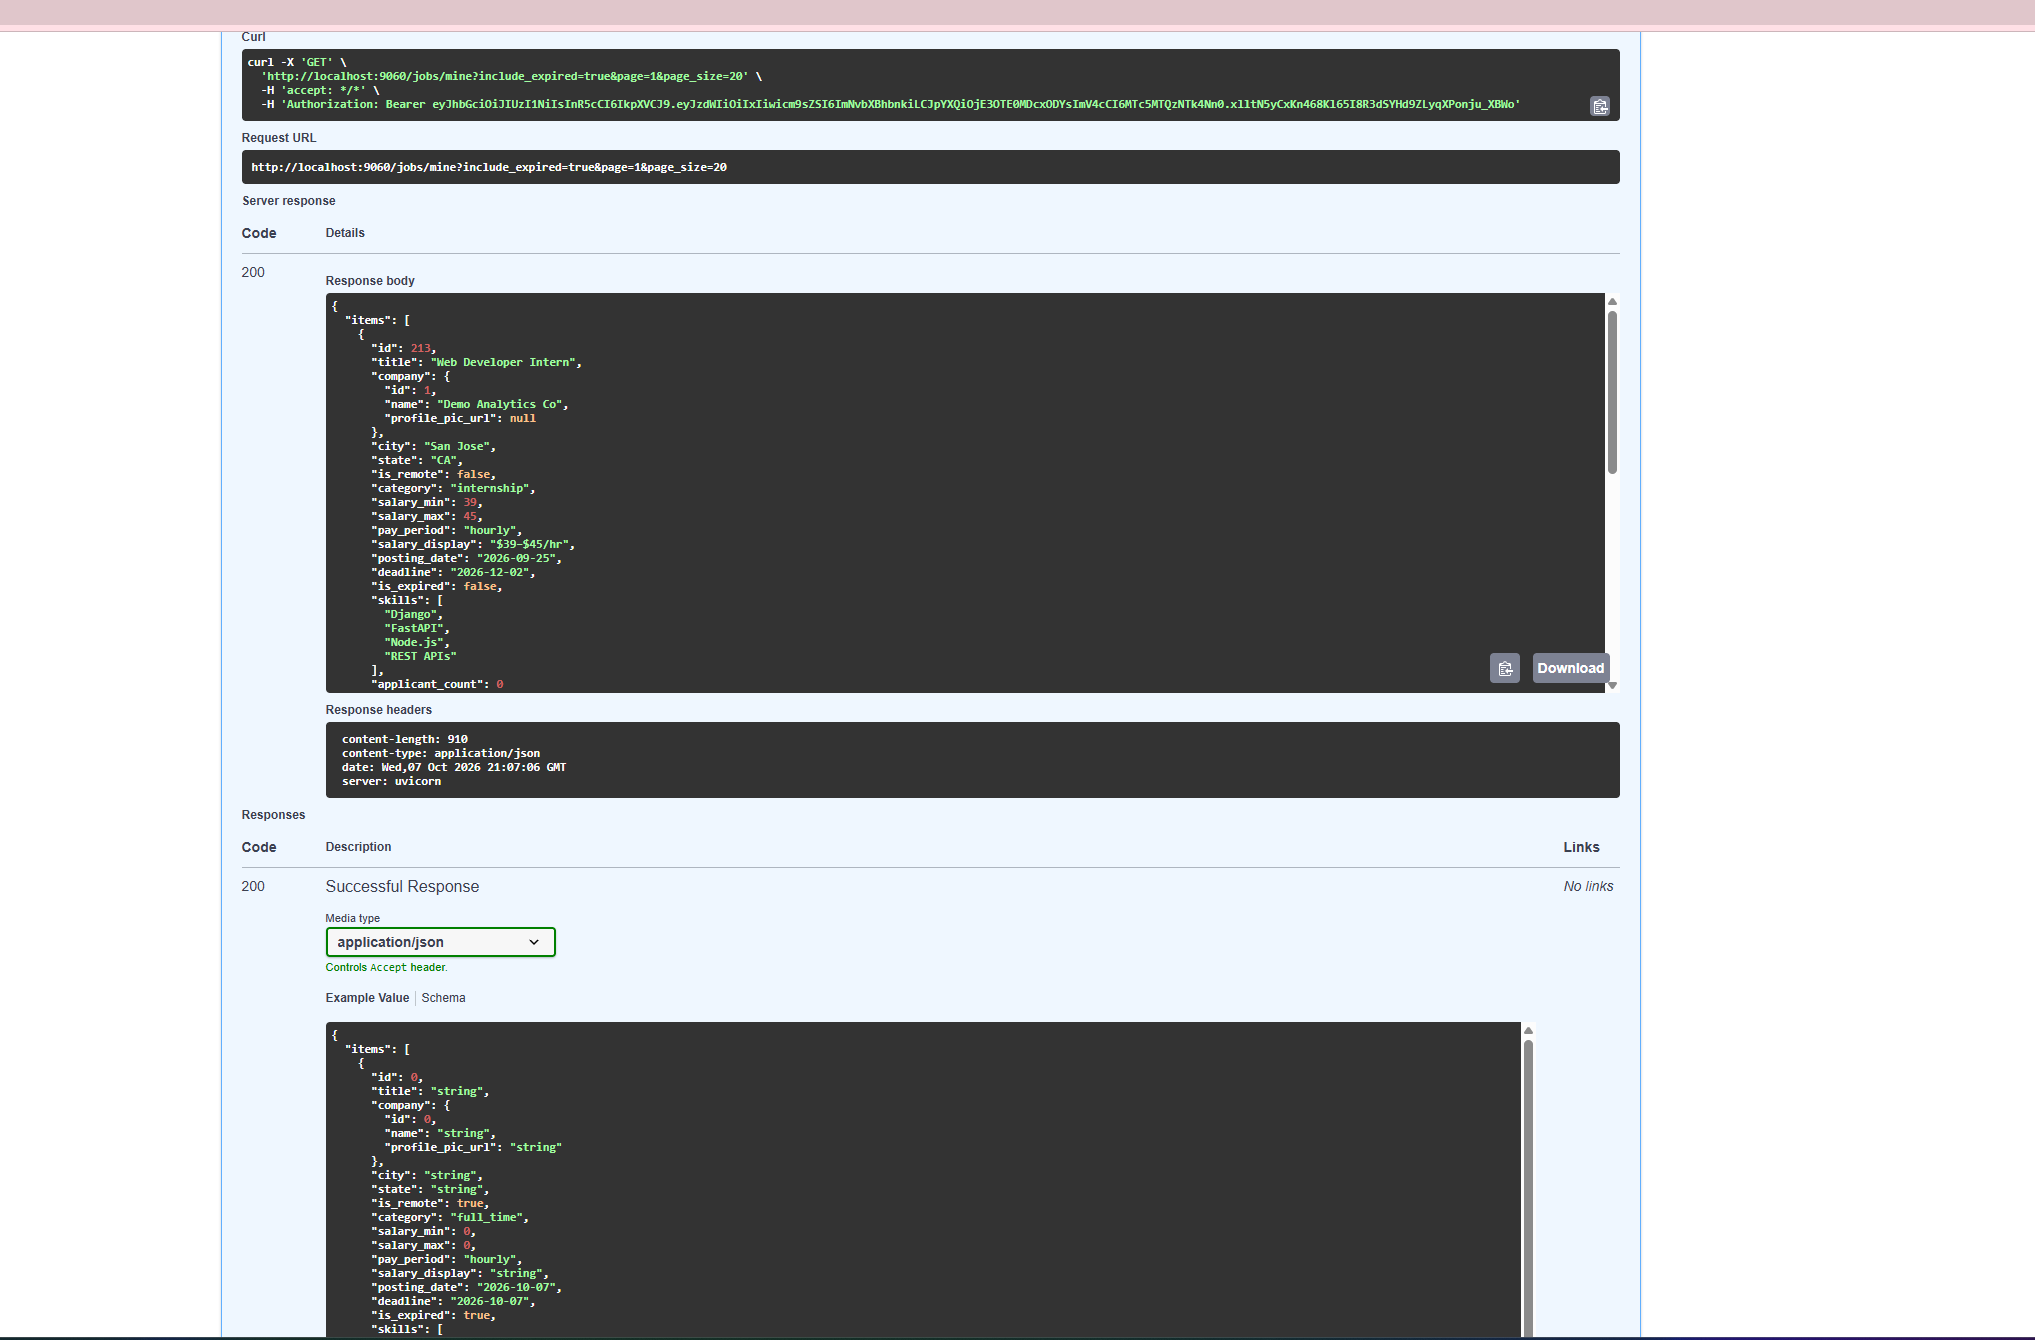
\includegraphics[width=\linewidth,height=0.42\textheight,keepaspectratio]{../screenshots/api_15_company_jobs_mine_200.png}
\caption{GET /jobs/mine}
\end{figure}

\begin{figure}[H]
\centering
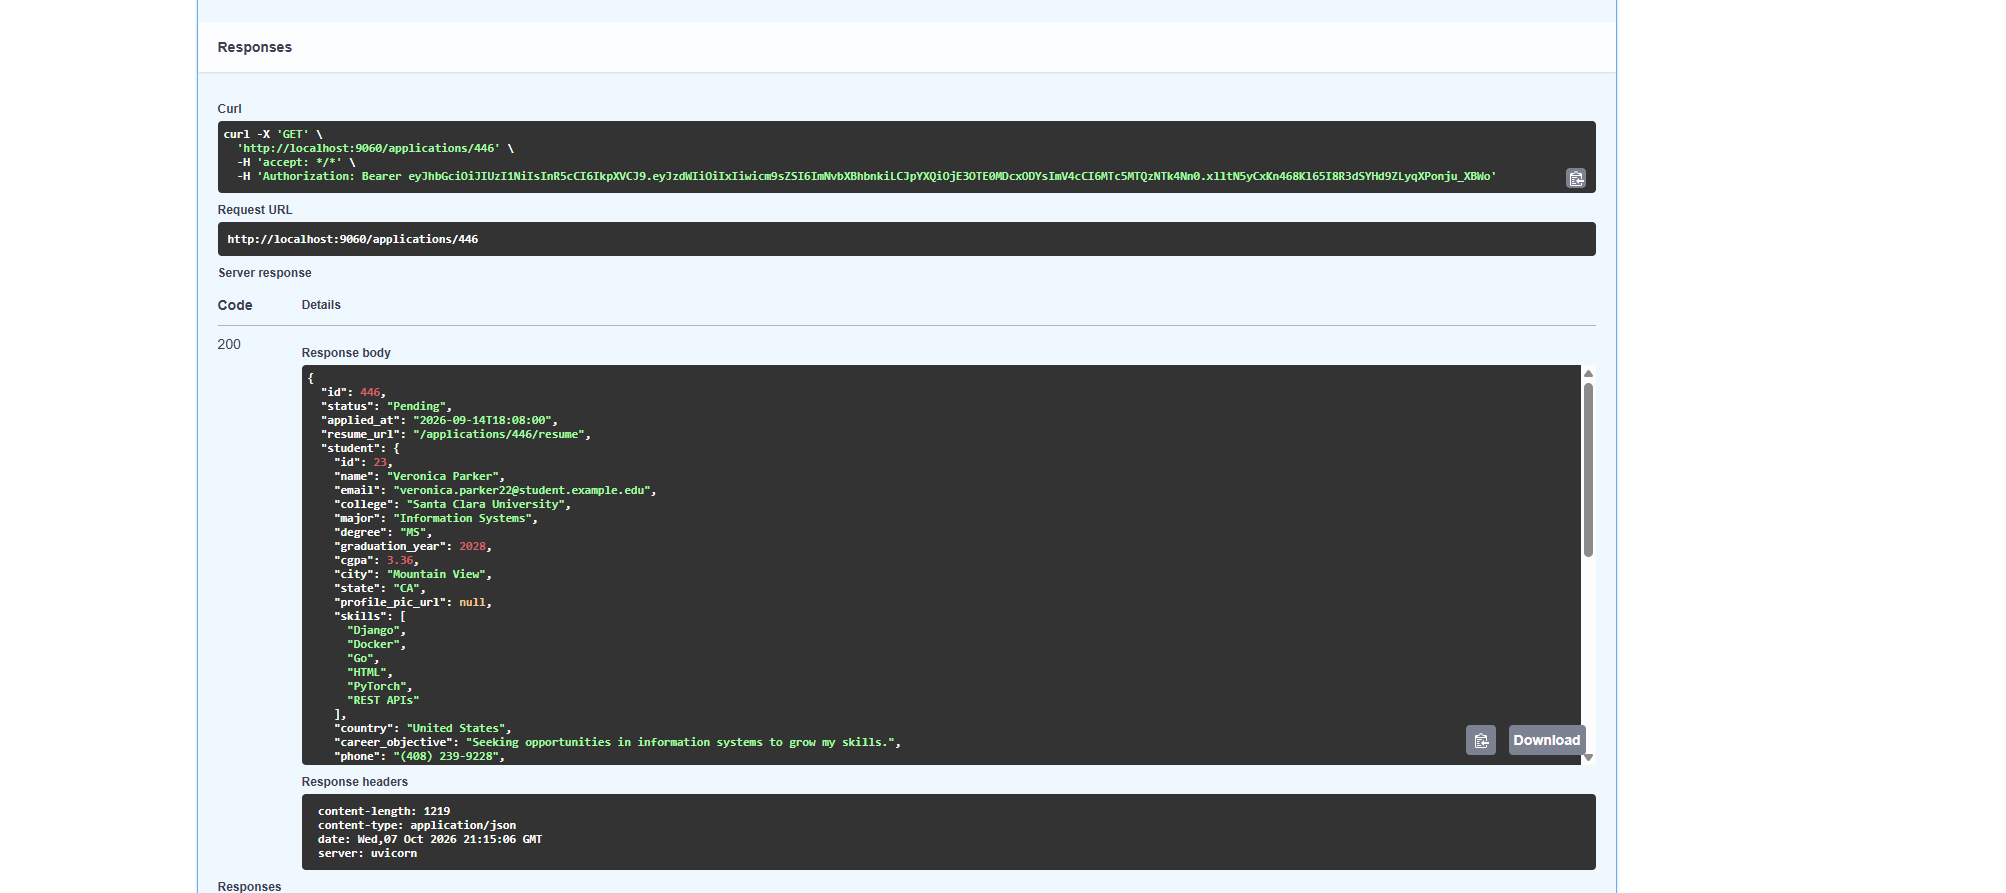
\includegraphics[width=\linewidth,height=0.42\textheight,keepaspectratio]{../screenshots/api_16_company_application_detail_200.png}
\caption{GET /applications/446 (applicant detail)}
\end{figure}

\begin{figure}[H]
\centering
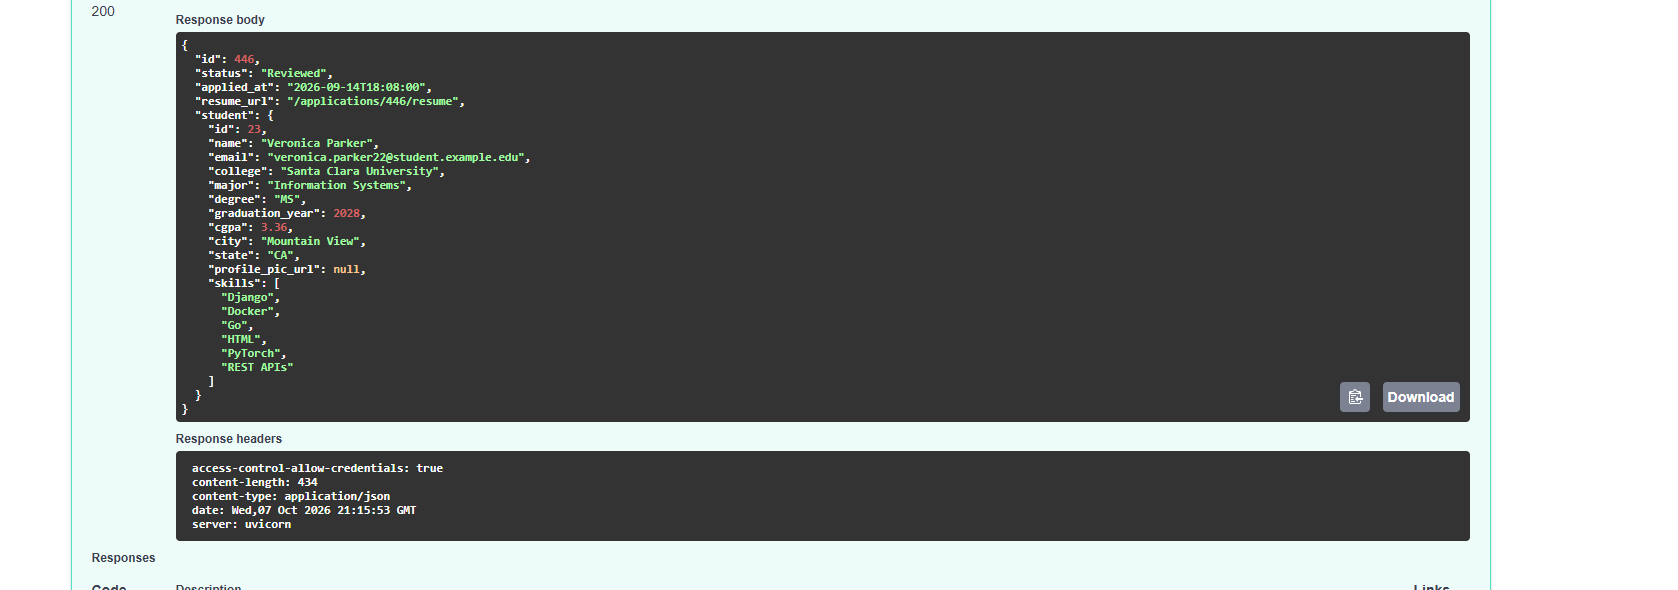
\includegraphics[width=\linewidth,height=0.42\textheight,keepaspectratio]{../screenshots/api_17_company_status_reviewed_200.png}
\caption{PATCH /applications/446/status sets Reviewed}
\end{figure}

\begin{figure}[H]
\centering
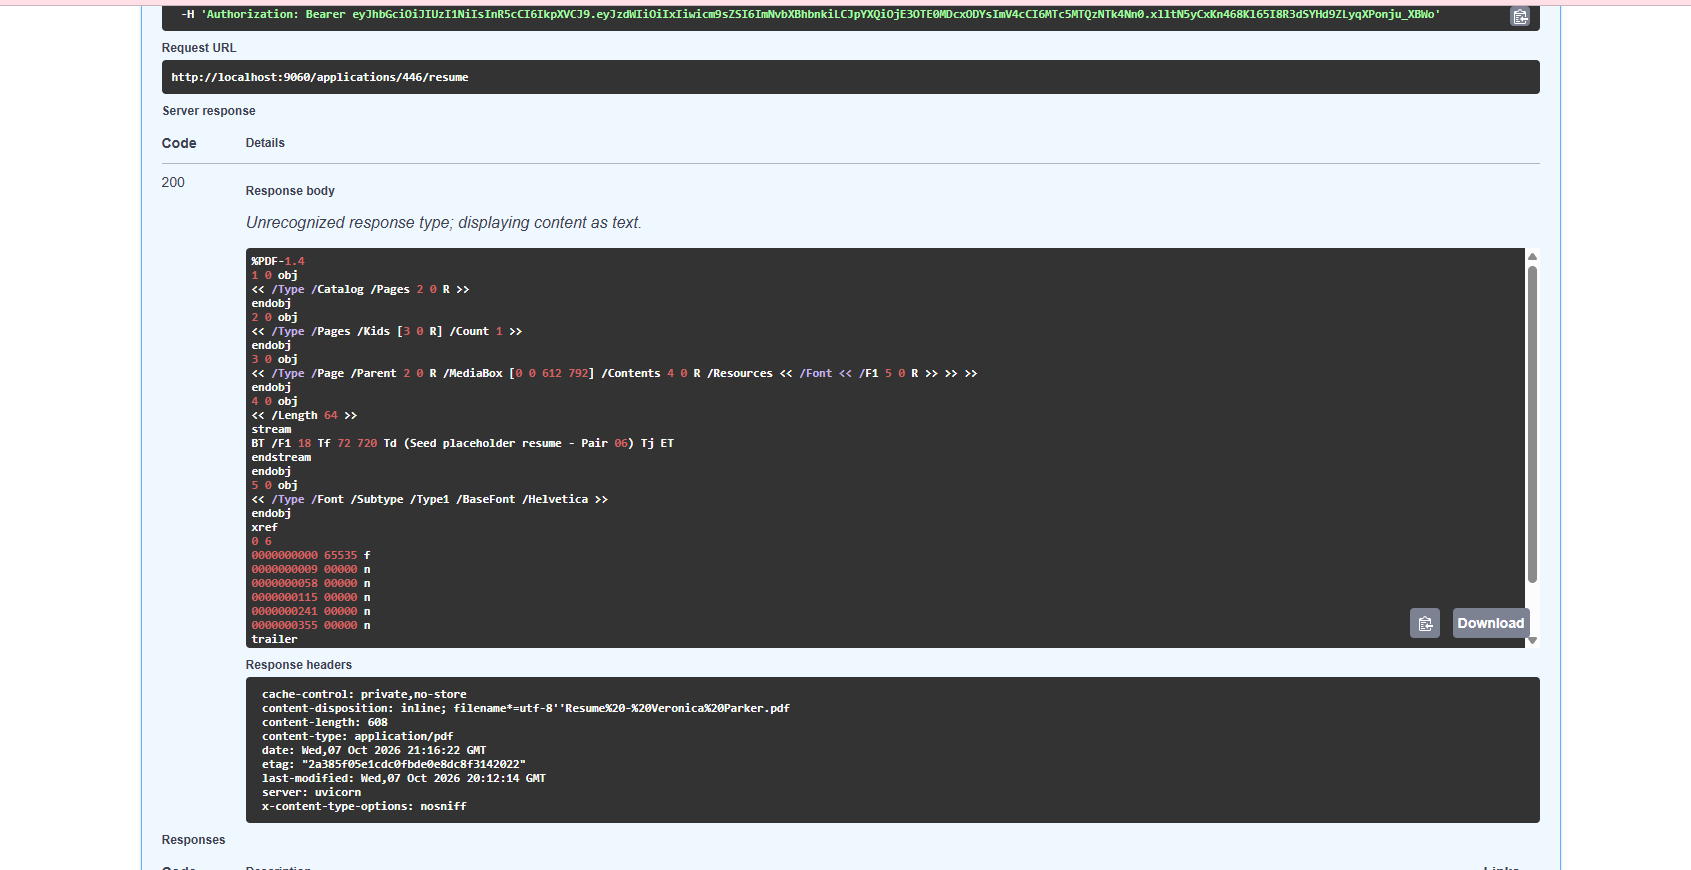
\includegraphics[width=\linewidth,height=0.42\textheight,keepaspectratio]{../screenshots/api_18_company_resume_pdf_200_private.png}
\caption{GET /applications/446/resume returns the PDF with private headers}
\end{figure}

\begin{figure}[H]
\centering
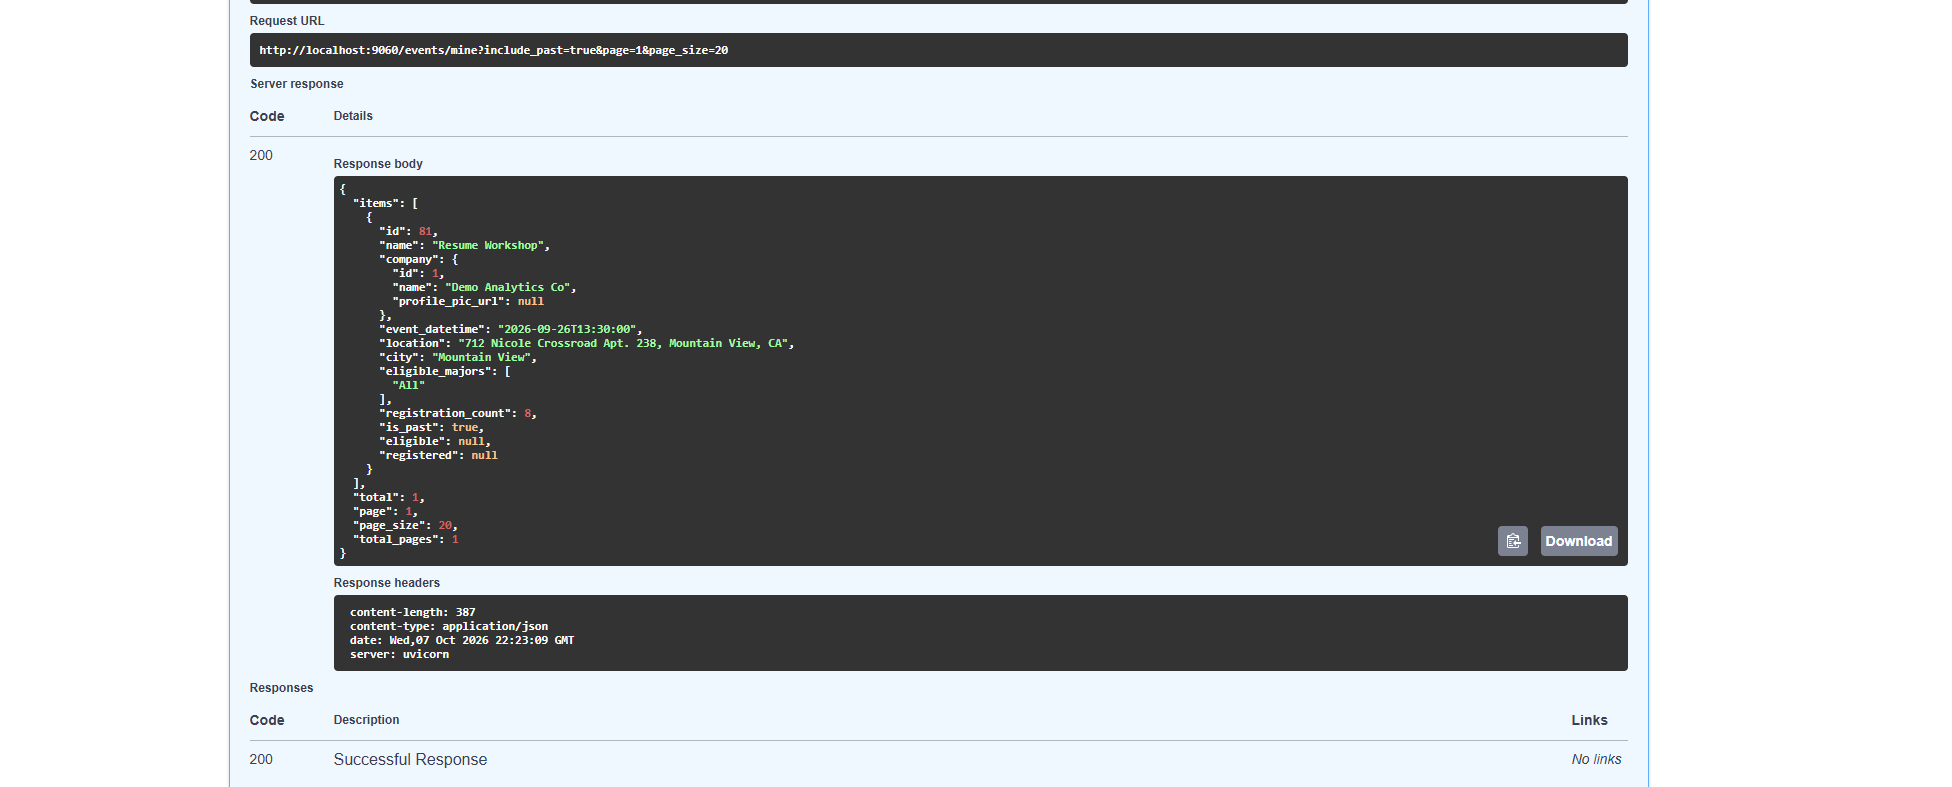
\includegraphics[width=\linewidth,height=0.42\textheight,keepaspectratio]{../screenshots/api_19_company_events_mine_200.png}
\caption{GET /events/mine}
\end{figure}

\begin{figure}[H]
\centering
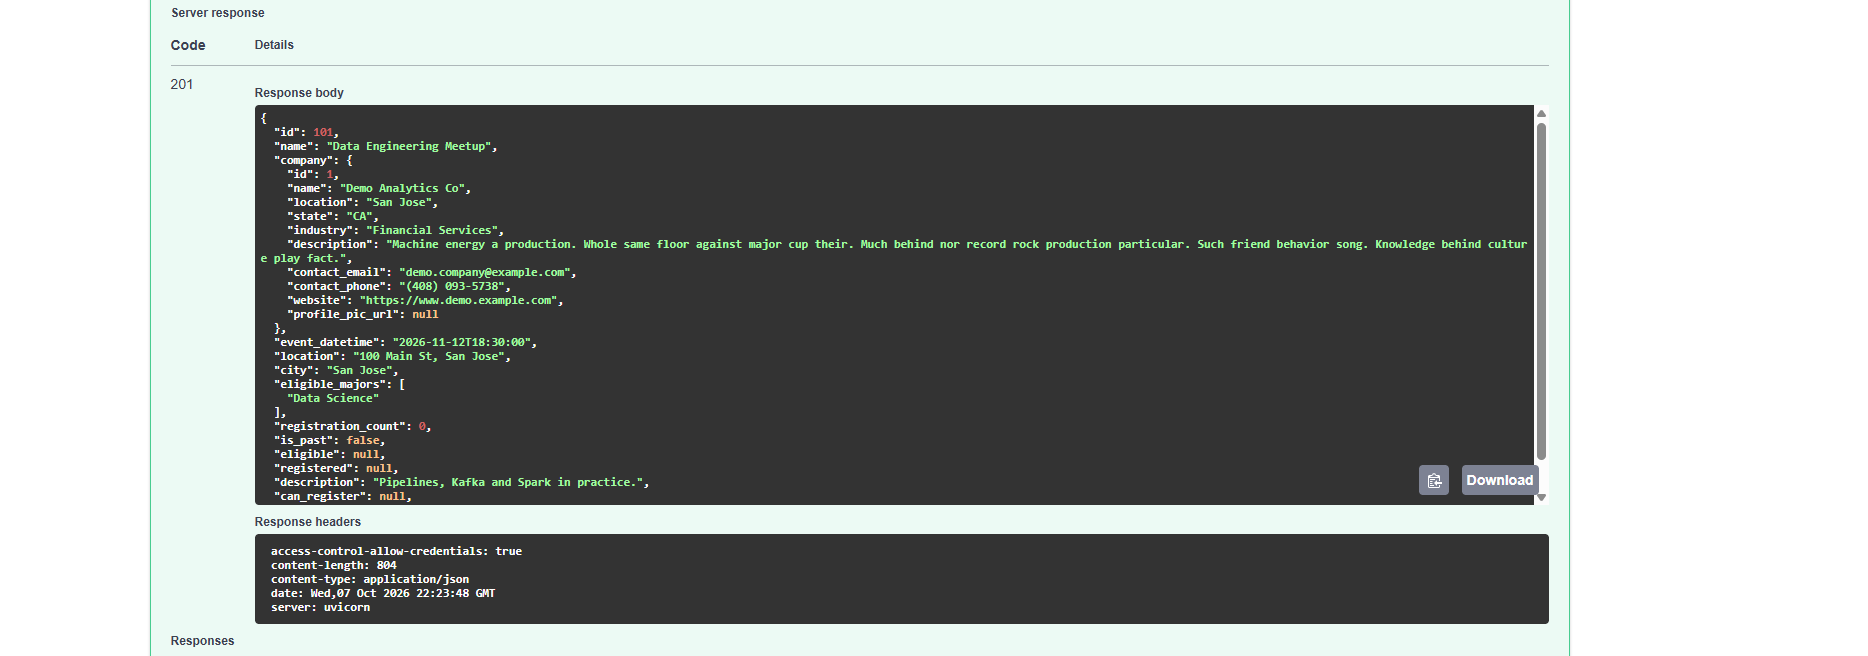
\includegraphics[width=\linewidth,height=0.42\textheight,keepaspectratio]{../screenshots/api_20_company_post_event_201.png}
\caption{POST /events returns 201}
\end{figure}

\subsection*{5.6 -- Tests, row counts and git history}

\pendingfigure{test\_\allowbreak{}01\_\allowbreak{}pytest\_\allowbreak{}summary.\allowbreak{}png}{pytest summary (346 passed)}

\pendingfigure{test\_\allowbreak{}02\_\allowbreak{}npm\_\allowbreak{}summary.\allowbreak{}png}{npm test summary (148 passed)}

\pendingfigure{db\_\allowbreak{}01\_\allowbreak{}row\_\allowbreak{}counts.\allowbreak{}png}{MySQL row counts for p06\_handshake}

\pendingfigure{git\_\allowbreak{}01\_\allowbreak{}history.\allowbreak{}png}{Git commit history showing both partners (taken last)}

A note on dates: the Swagger screenshots were taken on 6 to 7 October 2026 against a live database. Two of them (\code{api\_\allowbreak{}04}, application id 1501, and \code{api\_\allowbreak{}20}, event id 101) created extra rows, so the live database held 1,501 applications and 101 events at that time. The row counts in section 4 were measured later, after \code{python -\allowbreak{}m seed.\allowbreak{}generate\_\allowbreak{}seed -\allowbreak{}-\allowbreak{}reset} (RUN\_LOG start 2026-10-08 22:54), and show 1,500 and 100.

\section*{Section 6 -- API tests}

\subsection*{6.1 -- Swagger evidence}

Swagger UI (\code{http:\allowbreak{}/\allowbreak{}/\allowbreak{}localhost:\allowbreak{}9060/\allowbreak{}docs}) was used with the demo student and demo company logins. Each line says what the screenshot in section 5 proves. The Swagger set has no screenshot of a 401 or a 404; those two codes are covered by the pytest output in 6.2.

{\small
\begin{longtable}{>{\raggedright\arraybackslash}p{\dimexpr 0.486\linewidth-2\tabcolsep\relax}>{\raggedright\arraybackslash}p{\dimexpr 0.514\linewidth-2\tabcolsep\relax}}
\hline
\textbf{Screenshot} & \textbf{What it proves} \\ \hline
\endhead
\code{api\_\allowbreak{}01\_\allowbreak{}authorize\_\allowbreak{}dialog.\allowbreak{}png} & Bearer-token authentication is wired into Swagger: \code{POST /\allowbreak{}auth/\allowbreak{}login} takes \code{\{email,\allowbreak{} password,\allowbreak{} role\}} and the token goes into Authorize (value masked). \\ \hline
\code{api\_\allowbreak{}02\_\allowbreak{}jobs\_\allowbreak{}filters\_\allowbreak{}200.\allowbreak{}png} & \textbf{200}. Search and filters work together: \code{q=\allowbreak{}data science}, \code{category=\allowbreak{}internship}, \code{is\_\allowbreak{}remote=\allowbreak{}true}, \code{skills=\allowbreak{}Python\&skills=\allowbreak{}Machine Learning} (repeated keys), \code{skills\_\allowbreak{}match=\allowbreak{}any}, \code{include\_\allowbreak{}expired=\allowbreak{}false}; \code{total} is 3 with paging fields. \\ \hline
\code{api\_\allowbreak{}03\_\allowbreak{}student\_\allowbreak{}preferences\_\allowbreak{}200.\allowbreak{}png} & \textbf{200}. A student reads their own saved preferences (categories, cities, roles, minimum hourly rate, remote, event interests). This is the data the assistant's \code{get\_\allowbreak{}student\_\allowbreak{}preferences} tool reads. \\ \hline
\code{api\_\allowbreak{}04\_\allowbreak{}student\_\allowbreak{}apply\_\allowbreak{}201.\allowbreak{}png} & \textbf{201}. Multipart PDF upload creates an application with status \code{Pending}; the resume is exposed only as the protected path \code{/\allowbreak{}applications/\allowbreak{}1501/\allowbreak{}resume}. \\ \hline
\code{api\_\allowbreak{}05\_\allowbreak{}student\_\allowbreak{}my\_\allowbreak{}applications\_\allowbreak{}200.\allowbreak{}png} & \textbf{200}. A student lists only their own applications (total 11) with date, status (here \code{Reviewed}) and job summary. \\ \hline
\code{api\_\allowbreak{}06\_\allowbreak{}student\_\allowbreak{}events\_\allowbreak{}200.\allowbreak{}png} & \textbf{200}. Upcoming events (\code{include\_\allowbreak{}past=\allowbreak{}false}) with \code{registration\_\allowbreak{}count}, \code{eligible} and \code{registered} flags for the logged-in student. \\ \hline
\code{api\_\allowbreak{}07\_\allowbreak{}student\_\allowbreak{}events\_\allowbreak{}filtered\_\allowbreak{}200.\allowbreak{}png} & \textbf{200}. Event filters by \code{date\_\allowbreak{}from}, \code{date\_\allowbreak{}to} and \code{major}; 18 results. The last one shows \code{registered:\allowbreak{} true}. \\ \hline
\code{api\_\allowbreak{}08\_\allowbreak{}event\_\allowbreak{}register\_\allowbreak{}201.\allowbreak{}png} & \textbf{201}. Eligible student registers for event 59 (open to \code{All}). \\ \hline
\code{api\_\allowbreak{}09\_\allowbreak{}event\_\allowbreak{}register\_\allowbreak{}409\_\allowbreak{}duplicate.\allowbreak{}png} & \textbf{409} Conflict, \code{You are already registered for this event} (duplicate registration rule). \\ \hline
\code{api\_\allowbreak{}10\_\allowbreak{}event\_\allowbreak{}register\_\allowbreak{}403\_\allowbreak{}major.\allowbreak{}png} & \textbf{403} Forbidden, eligibility rule: the event is open to Computer Science and Marketing only and the student's major is Data Science. \\ \hline
\code{api\_\allowbreak{}11\_\allowbreak{}student\_\allowbreak{}directory\_\allowbreak{}peer\_\allowbreak{}no\_\allowbreak{}email.\allowbreak{}png} & \textbf{200}. \code{GET /\allowbreak{}students?major=\allowbreak{}Data Science} as a student: peer cards contain name, college, major, degree, graduation year, picture and skills, and no email, phone or GPA (total 25). \\ \hline
\code{api\_\allowbreak{}12\_\allowbreak{}student\_\allowbreak{}profile\_\allowbreak{}peer\_\allowbreak{}no\_\allowbreak{}email.\allowbreak{}png} & \textbf{200}. A student opening a peer profile gets the limited view plus career objective and experience; still no email, phone, GPA or date of birth. \\ \hline
\code{api\_\allowbreak{}13\_\allowbreak{}company\_\allowbreak{}students\_\allowbreak{}with\_\allowbreak{}email.\allowbreak{}png} & \textbf{200}. The same directory called with a company token includes \code{email} and \code{cgpa}. \\ \hline
\code{api\_\allowbreak{}14\_\allowbreak{}company\_\allowbreak{}student\_\allowbreak{}detail\_\allowbreak{}with\_\allowbreak{}email\_\allowbreak{}phone.\allowbreak{}png} & \textbf{200}. A company opening one student sees email, GPA and phone. The date of birth is not in the visible part of the body; its absence is checked by pytest (see 6.2). \\ \hline
\code{api\_\allowbreak{}15\_\allowbreak{}company\_\allowbreak{}jobs\_\allowbreak{}mine\_\allowbreak{}200.\allowbreak{}png} & \textbf{200}. A company lists only its own job postings, with \code{applicant\_\allowbreak{}count} (expired ones included because \code{include\_\allowbreak{}expired=\allowbreak{}true}). \\ \hline
\code{api\_\allowbreak{}16\_\allowbreak{}company\_\allowbreak{}application\_\allowbreak{}detail\_\allowbreak{}200.\allowbreak{}png} & \textbf{200}. Company opens applicant 446: status, resume URL and the student's profile with contact details. \\ \hline
\code{api\_\allowbreak{}17\_\allowbreak{}company\_\allowbreak{}status\_\allowbreak{}reviewed\_\allowbreak{}200.\allowbreak{}png} & \textbf{200}. \code{PATCH /\allowbreak{}applications/\allowbreak{}446/\allowbreak{}status} changes \code{Pending} to \code{Reviewed}. \\ \hline
\code{api\_\allowbreak{}18\_\allowbreak{}company\_\allowbreak{}resume\_\allowbreak{}pdf\_\allowbreak{}200\_\allowbreak{}private.\allowbreak{}png} & \textbf{200}. The resume is served only through the authenticated route: \code{content-\allowbreak{}type:\allowbreak{} application/\allowbreak{}pdf}, \code{cache-\allowbreak{}control:\allowbreak{} private,\allowbreak{} no-\allowbreak{}store}, \code{content-\allowbreak{}disposition:\allowbreak{} inline}, \code{x-\allowbreak{}content-\allowbreak{}type-\allowbreak{}options:\allowbreak{} nosniff}. The file is the seed's placeholder PDF. \\ \hline
\code{api\_\allowbreak{}19\_\allowbreak{}company\_\allowbreak{}events\_\allowbreak{}mine\_\allowbreak{}200.\allowbreak{}png} & \textbf{200}. A company lists only its own events (here one past event with 8 registrations). \\ \hline
\code{api\_\allowbreak{}20\_\allowbreak{}company\_\allowbreak{}post\_\allowbreak{}event\_\allowbreak{}201.\allowbreak{}png} & \textbf{201}. Company posts an event (id 101) restricted to \code{Data Science}; the response echoes the company and eligible majors. \\ \hline
\end{longtable}
}

\subsection*{6.2 -- Automated tests (pytest)}

Command: \code{python -\allowbreak{}m pytest -\allowbreak{}v} in \code{backend/\allowbreak{}}, on an in-memory SQLite database (never MySQL). The full verbose output is saved in \code{docs/\allowbreak{}part\_\allowbreak{}a\_\allowbreak{}tests.\allowbreak{}txt}. It was run on 2026-10-09 with Python 3.13.2 and pytest 8.3.3 and ends with:

\begin{lstlisting}
346 passed, 1 warning in 182.34s (0:03:02)
\end{lstlisting}

The earlier run recorded in \code{RUN\_\allowbreak{}LOG.\allowbreak{}txt} also passed 346 tests (216.73 s). Tests per file in \code{docs/\allowbreak{}part\_\allowbreak{}a\_\allowbreak{}tests.\allowbreak{}txt}:

{\small
\begin{longtable}{>{\raggedright\arraybackslash}p{\dimexpr 0.247\linewidth-2\tabcolsep\relax}>{\raggedleft\arraybackslash}p{\dimexpr 0.135\linewidth-2\tabcolsep\relax}>{\raggedright\arraybackslash}p{\dimexpr 0.618\linewidth-2\tabcolsep\relax}}
\hline
\textbf{File} & \textbf{Tests passed} & \textbf{Covers} \\ \hline
\endhead
\code{test\_\allowbreak{}applications.\allowbreak{}py} & 47 & Apply, resume rules, applicants, status, private resume route \\ \hline
\code{test\_\allowbreak{}assistant.\allowbreak{}py} & 12 & The \code{POST /\allowbreak{}assistant/\allowbreak{}chat} contract (placeholder reply, validation, student-only) \\ \hline
\code{test\_\allowbreak{}auth.\allowbreak{}py} & 22 & Signup, login, JWT checks, password rules \\ \hline
\code{test\_\allowbreak{}directory.\allowbreak{}py} & 26 & Student directory and the two role views \\ \hline
\code{test\_\allowbreak{}events.\allowbreak{}py} & 72 & Events, eligibility, registration, ownership \\ \hline
\code{test\_\allowbreak{}jobs.\allowbreak{}py} & 68 & Job postings, search and filters, ownership \\ \hline
\code{test\_\allowbreak{}preferences.\allowbreak{}py} & 33 & Saved preferences \\ \hline
\code{test\_\allowbreak{}profiles.\allowbreak{}py} & 66 & Profiles, pictures, email changes, public and private files \\ \hline
\textbf{Total} & \textbf{346} &  \\ \hline
\end{longtable}
}

The role-rule tests behind section 2.5 (each one passed in this run; the test names are in the table in 2.5):

{\small
\begin{longtable}{>{\raggedright\arraybackslash}p{\dimexpr 0.455\linewidth-2\tabcolsep\relax}>{\centering\arraybackslash}p{\dimexpr 0.091\linewidth-2\tabcolsep\relax}>{\raggedright\arraybackslash}p{\dimexpr 0.455\linewidth-2\tabcolsep\relax}}
\hline
\textbf{Rule} & \textbf{Status code} & \textbf{Test file and function} \\ \hline
\endhead
No token, garbage token, expired token, wrong secret, deleted account & 401 & \code{test\_\allowbreak{}auth.\allowbreak{}py:\allowbreak{}:\allowbreak{}test\_\allowbreak{}missing\_\allowbreak{}or\_\allowbreak{}garbage\_\allowbreak{}token\_\allowbreak{}is\_\allowbreak{}401}, \code{test\_\allowbreak{}expired\_\allowbreak{}token\_\allowbreak{}is\_\allowbreak{}401}, \code{test\_\allowbreak{}token\_\allowbreak{}signed\_\allowbreak{}with\_\allowbreak{}wrong\_\allowbreak{}secret\_\allowbreak{}is\_\allowbreak{}401}, \code{test\_\allowbreak{}token\_\allowbreak{}for\_\allowbreak{}deleted\_\allowbreak{}account\_\allowbreak{}is\_\allowbreak{}401} \\ \hline
Student calling a company-only endpoint, or the reverse & 403 & \code{test\_\allowbreak{}applications.\allowbreak{}py:\allowbreak{}:\allowbreak{}test\_\allowbreak{}applicant\_\allowbreak{}detail\_\allowbreak{}privacy}, \code{test\_\allowbreak{}jobs.\allowbreak{}py:\allowbreak{}:\allowbreak{}test\_\allowbreak{}cannot\_\allowbreak{}edit\_\allowbreak{}someone\_\allowbreak{}elses\_\allowbreak{}job\_\allowbreak{}or\_\allowbreak{}a\_\allowbreak{}missing\_\allowbreak{}job} \\ \hline
Another company's job posting or applicants & 403 & \code{test\_\allowbreak{}applications.\allowbreak{}py:\allowbreak{}:\allowbreak{}test\_\allowbreak{}applicants\_\allowbreak{}list\_\allowbreak{}is\_\allowbreak{}private\_\allowbreak{}to\_\allowbreak{}the\_\allowbreak{}job\_\allowbreak{}owner} \\ \hline
Another person's resume or application & 404 & \code{test\_\allowbreak{}applications.\allowbreak{}py:\allowbreak{}:\allowbreak{}test\_\allowbreak{}everyone\_\allowbreak{}else\_\allowbreak{}gets\_\allowbreak{}404\_\allowbreak{}for\_\allowbreak{}a\_\allowbreak{}resume}, \code{test\_\allowbreak{}applicant\_\allowbreak{}detail\_\allowbreak{}privacy} \\ \hline
Ineligible event registration & 403 & \code{test\_\allowbreak{}events.\allowbreak{}py:\allowbreak{}:\allowbreak{}test\_\allowbreak{}ineligible\_\allowbreak{}student\_\allowbreak{}is\_\allowbreak{}refused\_\allowbreak{}with\_\allowbreak{}a\_\allowbreak{}clear\_\allowbreak{}reason} \\ \hline
Duplicate application, registration or email & 409 & \code{test\_\allowbreak{}cannot\_\allowbreak{}apply\_\allowbreak{}twice\_\allowbreak{}but\_\allowbreak{}can\_\allowbreak{}apply\_\allowbreak{}to\_\allowbreak{}other\_\allowbreak{}jobs}, \code{test\_\allowbreak{}cannot\_\allowbreak{}register\_\allowbreak{}twice\_\allowbreak{}but\_\allowbreak{}others\_\allowbreak{}can}, \code{test\_\allowbreak{}duplicate\_\allowbreak{}email\_\allowbreak{}is\_\allowbreak{}rejected\_\allowbreak{}case\_\allowbreak{}insensitively} \\ \hline
Bad input is refused & 422 & \code{test\_\allowbreak{}applications.\allowbreak{}py:\allowbreak{}:\allowbreak{}test\_\allowbreak{}invalid\_\allowbreak{}status\_\allowbreak{}rejected[\allowbreak{}extra-\allowbreak{}field]\allowbreak{}} (unknown field), \code{test\_\allowbreak{}jobs.\allowbreak{}py:\allowbreak{}:\allowbreak{}test\_\allowbreak{}invalid\_\allowbreak{}edits\_\allowbreak{}rejected\_\allowbreak{}and\_\allowbreak{}change\_\allowbreak{}nothing}, \code{test\_\allowbreak{}events.\allowbreak{}py:\allowbreak{}:\allowbreak{}test\_\allowbreak{}invalid\_\allowbreak{}event\_\allowbreak{}rejected[\allowbreak{}.\allowbreak{}.\allowbreak{}.\allowbreak{}]\allowbreak{}} \\ \hline
Resume must really be a PDF, at most 5 MB & 4xx & \code{test\_\allowbreak{}non\_\allowbreak{}pdf\_\allowbreak{}uploads\_\allowbreak{}rejected[\allowbreak{}.\allowbreak{}.\allowbreak{}.\allowbreak{}]\allowbreak{}} (6 cases), \code{test\_\allowbreak{}resume\_\allowbreak{}over\_\allowbreak{}5mb\_\allowbreak{}rejected} \\ \hline
Company sees email and GPA but not phone or date of birth in the list; peers see neither & 200 & \code{test\_\allowbreak{}directory.\allowbreak{}py:\allowbreak{}:\allowbreak{}test\_\allowbreak{}company\_\allowbreak{}list\_\allowbreak{}shows\_\allowbreak{}contact\_\allowbreak{}and\_\allowbreak{}academic\_\allowbreak{}fields\_\allowbreak{}but\_\allowbreak{}never\_\allowbreak{}dob\_\allowbreak{}phone\_\allowbreak{}or\_\allowbreak{}password}, \code{test\_\allowbreak{}peers\_\allowbreak{}never\_\allowbreak{}get\_\allowbreak{}email\_\allowbreak{}phone\_\allowbreak{}gpa\_\allowbreak{}dob\_\allowbreak{}or\_\allowbreak{}city} \\ \hline
\end{longtable}
}

\subsection*{6.3 -- Front-end tests and API documentation}

\code{npm test} (Vitest, Testing Library, axios-mock-adapter) reported 14 test files and 148 tests passed in the run recorded in \code{METRICS.\allowbreak{}md} (16.69 s). It was not re-run for this report. API documentation exports are \code{docs/\allowbreak{}openapi.\allowbreak{}json} and \code{docs/\allowbreak{}postman\_\allowbreak{}collection.\allowbreak{}json}.

\section*{Section 7 -- Five transcripts}

% PARTNER (Parts B/C): paste the five transcripts here, from real runs
\textit{[To be added by Parts B and C from real runs.]}

\section*{Section 8 -- Reliability table}

% PARTNER (Parts B/C): valid and failed calls over 20+ turns, before and after repair, from real runs
\textit{[To be added by Parts B and C from real runs.]}

\section*{Section 9 -- Injection before and after}

% PARTNER (Parts B/C): the five verification queries before and after the defence, exactly what changed
\textit{[To be added by Parts B and C from real runs.]}

\section*{Section 10 -- Assistant tool-call evidence}

% PARTNER (Parts B/C): tool-call evidence from real runs
\textit{[To be added by Parts B and C from real runs.]}

\end{document}
